
%%==========================================================================================
%% Dokumenten- & Seitenlayout
%%==========================================================================================
%======================================================================
%	Vorlage
%======================================================================
%	$Id$
%	Matthias Kupfer
%======================================================================
%	Documentclass
%======================================================================
\documentclass[
%	draft,			% Entwurfsmodus: Bilder als Rahmen, Überlängen werden deutlich markiert
%	10pt,			% 
%	11pt,			% KOMA default
	12pt,			% 
	a4paper,		% DIN A4
	twoside,		% Zweiseitig
	german,			%
%----------------------------------------------------------------------
% Die folgenden Befehle stammen aus dem KOMA Paket
	headsepline,		% Linie unter der Kopfzeile	
%	headnosepline,		%
%	foodsepline,		% Linie über Fussnote	
	footnosepline=true,		%
	automark,		% Kolumnentitel lebendig
%	bigheadings,		% default: Überschriften gross setzen
%	headings=normal,		% Überschriften normal setzen
	smallheadings,		% Überschriften eher klein setzen
%	pointlessnumbers,	% Keinen Punkt hinter die letzte Zahl eines Kapitels (auch bei Anhang)
%	chapterprefix,		% Kapiteluberschriften "Kapitel"
	appendixprefix,		% Anhang
	openright,		% Kapitel auf der rechten (ungeraden) Seite anfangen lassen
%	openany,		% 
%	cleardoublestandard,	%
%	cleardoublepage=plain,	%
	cleardoubleempty,	% echt leere seiten zwischen kapiteln, keine seitenzahl
	abstracton,		%
	index=totoc,		% Index soll im Inhaltsverzeichnis auftauchen
	listof=totoc,		%
	bibliography=totoc,		%
%	parskip, 		% parskip-, parskip*, parskip+
% 	halfparskip, 		% halfparskip-, halfparskip* und halfparskip+
%	DIVclassic,
 	BCOR8mm,		%%?? Bindungskorrektur: 
				% BCOR<Breite des Bindungsverlustes> 
]{scrreprt} 

\setlength{\parindent}{0pt} % Absatzformatierung (Einrückung und Zeilenabstand)
\setlength{\parskip}{2ex} 

%======================================================================
%	Bearbeitung sowohl mit LaTeX als auch mit pdfLaTeX ermoeglichen
%======================================================================
%\newif\ifpdf 
	%\ifx\pdfoutput\undefined 
	%\pdffalse 			% we are not running pdflatex 
%\else 
	%\pdfoutput=1 			% we are running pdflatex 
	%\pdftrue 
%\fi


%======================================================================
%	Verwendete Pakete
%======================================================================

%\usepackage{babel}		% Sprachen

%% Latex mit deutschen Umlauten:
%% http://www.cs.albany.edu/~herrmann/latex_umlaute/

% \usepackage[latin1]{inputenc}   % Eingabe von ü,ö,ä,ß erlaubt 
\usepackage[utf8]{inputenc}


\usepackage[T1]{fontenc}	% EC-Schriften verwenden (vs. DC) da 8-Bit
				% EC-Schriften als T1-kodierten CM-Schriften
				% European/Ext.-Computer-Modern-(EC)-Schriften
				% Umlaute, Anführungszeichen ...
				% => Umlauten koennen richtig getrennt werden
				% FAQ 5.3.2
								
\usepackage{ae,aecompl}		% virtuelle-CM-Fonts
				% da EC nicht als PostScript-(Type-1) verfuegbar
				% => keine echten Umlaute im Dokument
				%(Problem bei Suche)
				% By loading the ae package (\usepackage{ae}), 
				% you loose some characters as mentioned in 
				% README. 
				% The package aecompl by Denis Roegel restores
				% these characters which are taken from the ec 
				% fonts. If you use pdftex, you will get these 
				% characters as bitmaps, but this might be 
				% better than not having them at all.

%\usepackage{times, mathptm}	% TimesNewRoman Schrift (Acrobat Reader Fonts), 
				% dazu braucht man auch den entsprechenden 
				% Zeichensatz für den Math-Mode
%\usepackage{pslatex}		% ? mathematische Formeln mit Standard 
				% Postscript Fonts gesetzt
			% Paket     Roman         Serifenlos  Typewriter
%\usepackage{times}	% -----------------------------------------------
			% times     Times         Helvetica   Courier
			% palatino  Palatino      Helvetica   Courier
			% newcent   NewCenturySch AvantGarde  Courier
			% bookman   Bookman       AvantGarde  Courier
			% Diese Schriften sind die Standard-PostScript-Schriften
			% und in jedem Drucker verfügbar

\usepackage{
%	german,			% Deutsche Trennungen (ALTE Rechtschreibung), 
				% Anführungsstriche und mehr 
	ngerman,		% Deutsche Trennungen (NEUE Rechtschreibung), 
				% Anführungsstriche und mehr
				%
%	acronym,		% Verwaltung von Abkuerzungen
	bibgerm,		% Deutsche Bibliographie; notwendig für Bibtex 
	calc,			% Erweiterung der arithmetischen Funktionen in 
				% LaTeX
				% wird verwendet um Titelseite zu zentrieren
	color,			% im Laufenden Text einfach mit \color{Farbe) zwischen den 
				% Farben umschalten, wobei Farbe einfach 
				% durch z.B. red, blue, black etc. ersetzt wird
				% \textcolor{farbe){Text)
%	epigraph,		% Zitat am Kapitelanfang
%	fancyhdr,		% Kopf- und Fußzeilen von Dokumenten frei 
				% gestalten
	fancybox,		% shadowbox, doublebox, ovalbox, Ovalbox 
	fancyvrb,		% verbatim Erweiterung:
	float,			% Positionierung von Gleitobjekten genau an der Stelle, wo man
				% 'figure'- oder 'table'-Umgebung die 
				% Positionierung [H] gesetzt werden
%	glosstex,		% Glossar und Abkürzungsverzeichnis
	mdwlist,		% compact list: itemize* ..
	scrdate,		% \todaysname 
	scrtime,		% \thistime
	scrpage2,		% Kopf- und Fußzeilen flexibel gestalten
				%
%	moreverb,		% verbatim-ähnlich: boxedverbatim, listing
%	verbatim,		% Darstellung von "Text, wie er eingegeben wird"
				%
%	lscape,			% Erstellt eine um 90% gedrehte *neue* Seite
%	textcomp,		% Sonderzeichen
	booktabs,		% Tabellenlinien
%	longtable,		% Tabellen > 1 Seite
%	supertabular,		% Tabellen > 1 Seite
	tabularx,		% Blocksatzspalten
    multirow,
%	ltxtable,		% tabularx + longtable
	multicol,		% mehrspaltige Zeilen
%	varioref,		% einheitliche Verweise
%	endnotes,		% Fussnoten -> Endnoten
%	rotating,		% sidewaystable und sidewaysfigure
%	natbib,			% Bibliographie ohne Klammer etc.
%	marvosym,		% Euro etc.
}

%\usepackage{pstricks}
\usepackage{listings}



%\usepackage{wasysym}

%\usepackage[german, first, bottomafter]{draftcopy}

%\usepackage{setspace}	% Durchschuß, Zeilenabstand
%\doublespace		% doppelzeilig oder
%\onehalfspacing	% anderthalbzeilig

% Für schöne Darstellung von Algorithmen
%\usepackage[german, algoruled, algochapter]{algorithm2e}
%\usepackage{algorithmic}
%\usepackage[chapter]{algorithm}
%\floatname{algorithm}{Algorithmus}

\usepackage{url}      		% irgendwas mit urls
\usepackage[table]{xcolor} % farbige Zeilen in Tabellen

%======================================================================
%	Bilder, Links
%======================================================================

\usepackage{graphicx}
\graphicspath{{img/}}	% Angabe der Pfade, wo die Grafiken liegen; mehrere Pfade sind möglich

\usepackage{thumbpdf}
\usepackage[
   colorlinks,        % Links ohne Umrandungen in zu wählender Farbe
   linkcolor=black,   % Farbe interner Verweise
   filecolor=black,   % Farbe externer Verweise
   citecolor=black,   % Farbe von Zitaten
   urlcolor=black
]{hyperref}

%======================================================================
%	Einstellungen
%======================================================================

%\typearea{11}		% Satzspiegel neu konstruieren (KOMA)
			%      10pt 11pt 12pt 
			% DIV : 8   10   12  

\pagestyle{scrheadings}	% Standart  Kopf- und Fußzeile
\setkomafont{pageheadfoot}{\small\scshape}

% ---------------------------------------------------------------------
%\setcounter{secnumdepth}{2}
%\setcounter{chapter}{-1}
\setcounter{tocdepth}{3}

% ---------------------------------------------------------------------
%\sloppy		% weniger Worttrennungen, größere Wortabstände
\fussy			% viele Worttrennungen, "schönere" Wortabstände

% ---------------------------------------------------------------------
%\flushbottom			% Ausrichtung der Seitenenden jeweils auf gleicher Höhe
\raggedbottom

% ---------------------------------------------------------------------
%\sloppypar		% Das hier relaxt die Einstellungen zum Wortabstand 
			% extrem. Damit ragen keine Worte über den rechten 
			% Zeilenabstand hinaus. Dafür muß stärker auf
			% Wortabstand geachtet werden, der kann dann ziemlich 
			% groß werden. Man erhält aber keine Meldung mehr 
			% über underfull boxes.

%Hiermit kann man das gleiche mit weniger Holzhammer erreichen:
%\setlength{\tolerance}{2000}           % Strafpunkt für Zeilenumbruch
%\setlength{\emergencystretch}{3pt}     % Soweit dürfen einzelne Worte mehr 
					% auseinandergezogen werden
%\setlength{\hfuzz}{1pt}                % Macht den rechten Rand um bis zu 1pt 
					% flatterig.

% ---------------------------------------------------------------------
%Vermeiden einzelner Zeilen am Ende einer Seite oder oben auf einer neuen Seite
\clubpenalty10000
\widowpenalty10000

% ----------------------------------------------------------------------
% neue Umgebungen für verwendete Sätze und Beispiele
\newtheorem{bsp}{Beispiel}[chapter]
\newtheorem{satz}{Satz}[chapter]

\lstset{
  language        = php,
  basicstyle      = \small\ttfamily,
  keywordstyle    = \color{blue},
  stringstyle     = \color{red},
  identifierstyle = \color{black},
  commentstyle    = \color{gray},
  showstringspaces=false,
  emph            =[1]{php},
  emphstyle       =[1]\color{black},
  emph            =[2]{if,and,or,else},
  emphstyle       =[2]\color{yellow},
  emph            =[3]{use, class, function, public, extends, \$this},
  emphstyle       =[3]\color{blue},
  emph            =[4]{\$modules},
  emphstyle       =[4]\color{blue}
}
\lstdefinelanguage{ned}
{
}
\lstset{
  language        = ned,
  basicstyle      = \small\ttfamily,
  keywordstyle    = \color{blue},
  stringstyle     = \color{red},
  identifierstyle = \color{black},
  commentstyle    = \color{gray},
  showstringspaces=false,
  emph            =[1]{simple, module, network, extends, channel, channelinterface,import,like,moduleinterface,package,property},
  emphstyle       =[1]\color{blue},
  emph            =[2]{if,and,or,else,for,input,output,inout, false,default,index,sizeof,true,typename,types},
  emphstyle       =[2]\color{yellow},
  emph            =[3]{types, parameters, gates, connections, submodules, allowunconnected},
  emphstyle       =[3]\color{orange},
  emph			  =[4]{int, string, double, @display, @class, volatile, xmldoc, xml, bool,const,this},
  emphstyle       =[4]\color{red}
}


%======================================================================
%	includeonly
%======================================================================

%\includeonly{		% Gibt an, welche Dateien der include-Befehl 
%			% tatsächlich einfuegen darf.
%  meta/metadaten		% Variablen setzen
%  ,titel		% Titelseite, Zusammenfassung und Inhaltsverzeichnis
% Alle per include einzulesenden Dateien müssen hier angegeben sein!
%  ,anleitung		% Anleitung zur Nutzung der Vorlage
%}

% Aufteilung der Arbeit in folgende Bestandteile in angeg. Reihenfolge
%
% Titelseite
% Bibliographische Beschreibung (Rückseite der Titelseite)
% (Aufgabenstellung)
% Danksagung
% Abstract
% Inhaltsverzeichnis
% Tabellenverzeichnis
% Abbildungsverzeichnis
% Einleitung
% Inhalt
% Zusammenfassung/Ausblick
% (Verzeichnis verwendeter Terme)
% Arbeitsaufteilung
% Glossar (Abkürzungsverzeichnis)
% (Index)
% Literaturverzeichnis
% (Thesen)
% (Selbstständigkeitserklärung)
% Anhänge

\begin{document}
	%%========================================================================================
	%% Variablen, \hypersetup, etc
	%%========================================================================================
	%======================================================================
%	Metadaten
%======================================================================
%	$Id$
%	Matthias Kupfer
%======================================================================

\newcommand{\dcsubject}{Bachelorarbeit}
% z.B. (Diplom/Studien/Haus)arbeit, Praktikumsbericht, Studie, Beleg, 
% (Pro/Haupt/Ober)seminar, Seminar usw.
\newcommand{\dctitle}{Integration von Umwelt- und Sensormodellierung in die Netzwerksimulation}
\newcommand{\dcsubtitle}{~} % Untertitel, falls erforderlich

\newcommand{\dcauthorlastname}{Thomas Rückert}
\newcommand{\dcauthorfirstname}{}

\newcommand{\dcauthoremail}{thomas.rueckert@s2010.tu-chemnitz.de} 
\newcommand{\dcdate}{\today} 

\newcommand{\dcplace}{Chemnitz} % Ort, kann an der TU meist so bleiben
\newcommand{\dcuni}{Technische Universität \dcplace}
\newcommand{\dcdepart}{Fakultät für Informatik} % Fakultätsangabe
\newcommand{\dcprof}{Professur für Technische Informatik} % Angabe der Professur

\newcommand{\dcpruefer}{Prof. Dr. Wolfram Hardt}% Prüfer der Arbeit
\newcommand{\dcadvisor}{Dipl.-Inf. Mirko Lippmann}% Betreuer der Arbeit

\newcommand{\dckeywords}{Liste,von,Stichworten,die,als,Schlagworte,geeignet,
sind}

%%======================================================================
% Einstellungen des Hyperref-Paketes
\hypersetup{%    
	pdftitle	= {\dctitle}, %
	pdfsubject	= {\dcsubject, \dcdate}, %
	pdfauthor	= {\dcauthorfirstname~\dcauthorlastname, \dcauthoremail}, %
	pdfkeywords	= {\dckeywords}, %
	pdfcreator	= {pdfTeX with Hyperref and Thumbpdf}, %
	pdfproducer	= {LaTeX, hyperref, thumbpdf}, %
	% weitere PDF-Einstellungen in hyperref.cfg
}
%%======================================================================

	%%========================================================================================
	%% formaler Aufbau - Anfang
	%%========================================================================================
	%======================================================================
%	Titelseite 
%======================================================================
%	$Date:$
%	$Revision:$
%	Matthias Kupfer
%======================================================================

%%======================================================================
%% Schmutztitel
%%======================================================================
%\extratitle{
%	\usekomafont{sectioning}\mdseries 
%	\begin{center}
%		\Huge \dcsubject\\[1.5ex]
%		\hrule
%		\vspace*{\fill}
%		
\includegraphics{TUC_deutsch_einzeile_CMYK}
%	\end{center}
%}

%%======================================================================
%% Titelkopf
%%======================================================================
\titlehead{
	\vspace*{-1.5cm}
	% Schriftfamilie wie alle Überschriften, aber nicht fett
	\usekomafont{disposition}\mdseries 
	\begin{center}
		\raisebox{-1ex}{
\includegraphics[scale=1.4]{TUC_deutsch_einzeile_CMYK}}\\
		\hrulefill \\[1em]
		{\Large\dcdepart}\\[0.5em] 
		\dcprof
	\end{center}
	\vspace*{1.5cm}
}

%%======================================================================
%% Subjekt
%%======================================================================
\subject{\bf\Huge\dcsubject}


%%======================================================================
%% Titel
%%======================================================================
\title{\sf\Large
	\dctitle
	\\
	\dcsubtitle
}

%%======================================================================
%% Autor des Dokumentes
%%======================================================================
\author{\dcauthorfirstname~\dcauthorlastname}
	
%%======================================================================
%% Ort, Datum
%%======================================================================
\date{\dcplace, den \dcdate
}

%%======================================================================
%% Publishers
%%======================================================================
\publishers{
	{\parbox{\textwidth-8em}{
		\begin{tabbing}
			{\bf Betreuer:}\quad\=\kill
			{\bf Prüfer:}	\>\dcpruefer\\
			{\bf Betreuer:}	\>\dcadvisor
		\end{tabbing}	
	}}
}

%%======================================================================
%% bibliografische Angaben
%%======================================================================
\lowertitleback{
\textbf{\dcauthorlastname, \dcauthorfirstname}\\
\dctitle\\
\dcsubject,~\dcdepart\\
\dcuni,~\ifcase\month\or
  Januar\or Februar\or März\or April\or Mai\or Juni\or
    Juli\or August\or September\or Oktober\or November\or Dezember\fi
    ~\number\year
}

%%======================================================================
%% maketitle
%%======================================================================

\maketitle 
	\def\abstractname{Abstract} 	% Wenn der Text "Zusammenfassung" erscheinen soll, dann muß dies auskommentiert werden
				
\begin{abstract}
%%
%% Inhalt der Arbeit
%%
In dieser Arbeit soll die Simulation von Sensorknoten in einem Netzwerk untersucht werden. Dabei sollte zum einen die Kommunikation zwischen den verschiedenen Knoten, von denen es viele und verschiedene geben soll betrachtet. Diese führen eine kabellose Kommunikation miteinander. 
Die einzelnen Konten besitzen Sensoren, die verschiedene Umweltparameter auslesen. Die Bereitstellung dieser Umweltparameter in der Simulationsumgebung ist auch ein Teil der Implementierung. Außerdem sind die Knoten batteriebetrieben und deren Energieverwaltung wurde betrachtet. Nach Test und Modellierung ist die Auswertung und Visualisierung von Simulationsdaten von entscheidender Rolle. 
Als Simulationsumgebung und -sprache wurde Omnet++ mit dem Framework MiXiM genutzt, welches Grundfunktionen für mobile Knoten mit kabelloser Kommunikation bereit stellt.
\end{abstract} 
	\cleardoubleemptypage
\pagenumbering{roman}
\pdfbookmark{Inhaltsverzeichnis}{Inhaltsverzeichnis}
\tableofcontents
	\cleardoublepage
\markboth{Abbildungsverzeichnis}{Abbildungsverzeichnis}
\listoffigures
	\cleardoublepage
\markboth{Tabellenverzeichnis}{Tabellenverzeichnis}
\listoftables
	%%\renewcommand{\listalgorithmname}{Algorithmenverzeichnis}
%\cleardoublepage
%\addcontentsline{toc}{chapter}{Algorithmenverzeichnis}
%\listofalgorithms
	%%\cleardoublepage
%\addcontentsline{toc}{chapter}{Abkürzungsverzeichnis}
%\markboth{Abk"urzungsverzeichnis}{Abk"urzungsverzeichnis}
%\def\listacronymname{Abk"urzungsverzeichnis}
%\printglosstex(acr)
	
	%%========================================================================================
	%% Verzeichnissauflistung mit weißer Seite abschließen und danach Seitennummerierung bei 1
	%%========================================================================================
	\cleardoublepage
\pagenumbering{arabic}
\setcounter{page}{1}

	%%========================================================================================	
	%% I N H A L T 	
	%%========================================================================================
	\chapter{Einleitung}

Die Verwendung von Sensoren steigt in der heutigen Zeit mehr und mehr an. Sensorknoten unterscheiden sich im Kern nicht von herkömmlichen Computern und sind zusätzlich mit Sensoren und oft mit Batterien und Funkmodulen ausgestattet. Da Computerbauteile bei gleicher Leistung kleiner und kleiner werden, ist es nicht verwunderlich, dass auch Sensorknoten immer weiter schrumpfen. Mit kleinen Knoten im Millimeterbereich zu geringen Kosten ist es möglich sehr große Netzwerke von Sensoren zu erschaffen, die miteinander kommunizieren. So können beispielsweise die Umgebungsparameter großer Naturflächen detailliert untersucht werden, ohne dass eine große Forschungsstation aufgebaut werden müsste. Stattdessen kann man viele kleine Sensorknoten in der Umwelt verteilen, die miteinander in Kontakt stehen. \newline

\chapter{Motivation}

Diese Sensorknoten werden sinnvollerweise in drahtlosen Sensornetzwerken organisiert. Das Netzwerk dient dabei dem Sammeln von Daten, also dem Senden von den Messdaten zu einer Datensenke. Da der Energiehaushalt bei Sensorknoten meist sehr sensibel ist, kommt neben einem Funktransceiver oft auch ein Wake-up-Receiver zum Einsatz.\\
Diese Netze müssen vor dem Praxiseinsatz getestet werden, wobei die Betrachtung des Energiezustands über lange Zeiträume bei verschiedenen Routingverfahren von Bedeutung ist und wie sich die Knoten in großen Netzen von tausenden Knoten verhalten.\\
Das Ziel dieser Arbeit ist es, neben der Simulation von den Netzwerken das Verhalten der Sensorik abbilden zu können. Diesen sollen Umgebungsparameter bereitgestellt werden. Dabei ist wiederum die Betrachtung des Energiehaushalts von entscheidender Bedeutung. Für Nutzung großer Netzwerke sollen Möglichkeiten bereitgestellt werden, die statistischen Daten von den Simulationen zu visualisieren, damit diese bestmöglich ausgewertet werden können.\\
Zuletzt soll anhand von Tests und Beispielanwendungen gezeigt werden, wie die Implementierung der Sensormodelle genutzt werden könnte.
    \chapter{Vorbetrachtungen}

Im folgenden werden die verwendeten Technologien betrachtet. Als Versionsverwaltungssoftware wurde Git\cite{git} auf der Platform Github\cite{github} verwendet, worauf nicht weiter eingegangen wird. Zum Erstellen der Simulation wurde Omnet++\cite{omnet} mithilfe des MiXiM-Frameworks\cite{mixim} benutzt.

\section{Evaluation von Systemen}

Im Entwicklungsprozess eines jeden Systems müssen neue Teile oder Module evaluiert werden. Für das Testen gibt es verschiedene Möglichkeiten, die einem zur Verfügung stehen. Im frühen Stadium der Entwicklung bietet das Abschätzen ohne Implementierung und daher ohne zu messen eine kostengünstige Variante zum Bestimmen von Designparametern. Allerdings sind diese Ergebnisse oftmals sehr grob und es lässt sich auch nicht jeder Wert so einfach bestimmen. \newline
Es ist daher notwendig genauere Tests durchzuführen. Wenn man ein komplett implementiertes und produziertes System anschließend testen möchte kann das sehr teuer werden, sollten viele Fehler auftreten oder wenn man merkt, dass die Implementierung wohl doch nicht die Optimale für ein gewünschtes Ziel ist. \newline
Man kann diesen Problemen zuvor kommen, indem man noch vor der ersten Implementierung eines Systems Simulationen und Emulationen erstellt und Prototypen anfertigt. Das senkt die Kosten mitunter erheblich und es lassen sich beinahe alle Parameter des zukünftigen Produkts überprüfen, auch wenn es das Testen des fertigen Produkts nicht komplett ersetzen kann.

\todo{überarbeiten}

\paragraph{Simulation}

Eine Simulation ist ein Modell eines Systems, welches dieses passend abbildet. Mit diesem Modell kann herausgefunden werden, was im realen System später umsetzbar ist. Der Zustand eines solchen Modells ändert sich im Laufe der (Simulations-)Zeit. Daher führt das Modell Zustandsübergange durch, welche als Events bezeichnet werden. Man kann Systeme nach den Zeitpunkten an denen Zustandswechsel möglich sind, in analoge und diskrete unterteilen. Wie der Name vermuten lässt können im analogen Fall zu jeder Zeit Zustandsübergänge stattfinden, im diskreten dagegen nur zu bestimmten Zeitpunkten.

\paragraph{Emulationen}

Eine Emulation ist die Implementierung eines Systems, welche den kompletten Funktionsumfang des Entwurfs abdeckt. Diese kann mit einer Hardwarebeschreibungssprache wie VHDL definiert werden und auf einem FPGA oder innerhalb eines Netzwerks von FPGAs ausgeführt werden. Man spricht daher von einer homogenen Hardwareplattform.

\paragraph{(Rapid) Prototyping}

Ein Prototyp ist ebenfalls eine Implementierung eines Systems, die den kompletten Funktionsumfang des Entwurfs abdeckt, allerdings geringere Anforderungen and Timing, Größe und Kosten stellt. Prototypen zum Beispiel oftmals wesentlich größer als das Endprodukt. Wenn er alle sonstigen Anforderungen zur Genüge erfüllt, so kann er in das finale Design umgewandelt werden und verliert bei diesem Prozess alle Grenzen des Prototyps. Im Gegensatz zur Emulation kommt eine heterogene Hardwareplattform zum Einsatz. So können etwa fertige Prozessoren, Speicher, weiterhin FPGAs oder spezielle Chips wie ein ASIC zum Einsatz kommen.

\endgraf

Für die Arbeit ist die Entscheidung auf eine Simulation gefallen. Man kann sich dabei auf die wesentlichen Funktionen konzentrieren und grundsätzliche Überlegungen über die genaue Umsetzung von gewissen Bauteilen zunächst außer Acht lassen. Ein Modell muss stets nur so genau spezifiziert werden wie nötig und so gut wie nie mit der Komplexität der Realität übereinstimmen. \newline
Der Fokus der Arbeit liegt daher auch auf dem Verwalten von Umweltparametern, der Erfassung dieser durch Sensoren auf vielen verschiedenen Sensorknoten und nicht darauf, wie die einzelnen Bauteile technisch aufgebaut sein könnten oder sollten. 

\section{Sensoren}

Den Hauptgegenstand in der Simulation bilden Sensoren, welche auf Sensorknoten angebracht sind. Ein solcher Knoten kann dann wiederum ein oder mehrere Sensoren besitzen.\newline
Sensoren sind das technische Gegenstück zu den menschlichen Sinnen, denn sie können physikalische oder chemische Eigenschaften wahrnehmen. Dabei arbeiten Sensoren allerdings noch wesentlich genauer, denn es lassen sich Messgrößen quantitativ exakt bestimmen.\newline

\todo{allgemeines Modell Sensor}



Allgemein ist ein Sensor wie in Abbildung \ref{fig:fff} aufgebaut. Die SensingUnit, zu deutsch Aufnehmer, ist dabei das Herzstück, denn es ist das Bauteil, in dem der gesuchte Wert aus der Umgebung aufgenommen wird. Je nach Sensor ist dieser Wert jedoch nicht direkt interpretierbar. Das Signal wird daher zunächst aufbereitet. Zum einen kann das bedeuten, falls der Messimpuls nur sehr kurz war, diesen zu verlängern, sodass folgende Bauteile verwertbare Eingaben bekommen können. Zum anderen kann es nötig sein, dass ein analoges in ein digitales Signal umgewandelt werden muss. Diese Aufgaben werden durch Signalformer und Signalwandler übernommen.\newline
Zuletzt muss das Signal noch durch einen Messumformer aus einem bloßen digitalen Wert ohne direkte Bedeutung in einen Messwert in der benötigten Messeinheit umgewandelt werden. Dieser Wert kann dann über eine Schnittstelle nach außen gegeben werden und von anderen Teilen auf einem Sensorknoten verarbeitet werden.

\subsection{Beispiele für Sensoren}

Im folgenden Abschnitt werden ein paar verschiedene Beispiele für Sensoren vorgestellt. Es wird für die in der Implementierung umgesetzten Sensoren für Temperatur, Helligkeit, Luftdruck und Luftfeuchtigkeit jeweils ein Beispiel erläutert.

\paragraph{Temperatur}

Vermutlich bedingt durch die große Verbreitung und die bereits lange Existenz von Temperaturfühlern gibt es eine sehr hohe Zahl verschiedener Möglichkeiten Temperatur zu messen, wobei sich die verschiedenen Umsetzung zum Teil auch sehr stark unterscheiden. Dabei gibt es sowohl Sensoren mit passiven, als auch mit aktiven Aufnehmern.\newline
Ein Beispiel für eine Umsetzung ist ein Temperatursensor mit Aufnehmer in Form eines Heißleiters. Dieser verringert seinen Widerstand, wenn seine Temperatur steigt. Es kann nun eine stets konstante Spannung an den Heißleiter angelegt werden, um auf die Temperatur des Bauteils zu schließen. Da zum abgreifen der Messwerte eine Spannung von außen angelegt werden muss, liegt ein passiver Aufnehmer vor.

\begin{figure}[htbp]
\centering
\caption{Deutschlandkarte der mittleren Temperatur zwischen 1961 und 1990}
\label{fig:temperatur}
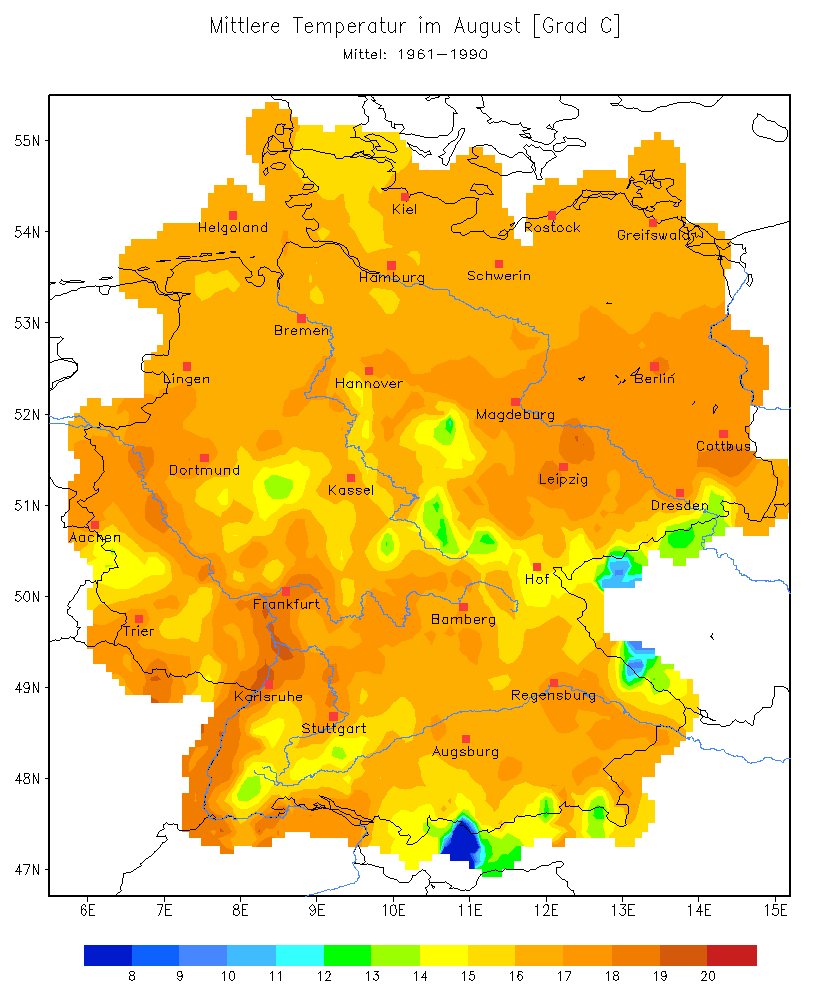
\includegraphics[width=\textwidth]{temperatur}
\end{figure}

\paragraph{Helligkeit}

Ein Lichtsensor oder auch Photodetektor dient dazu, um die stärke des einfallenden Lichts zu bestimmen, also die Helligkeit. Diese können unter Nutzung des photoelektrischen Effekts ganz ähnlich zum vorgestellten Temperatursensor mit Heißleiter genutzt werden. Die sogenannte Photoleitung bezeichnet hierbei die Zunahme der Leitfähigkeit, durch steigende Bestrahlung. Um den Sensor mit einem aktiven Aufnehmer zu nutzen, kann ein Sensor auch mit dem photovoltaische Effekt gebaut werden. Dieser wird ebenfalls bei der Gewinnung von elektrischer Energie durch das Sonnenlicht benutzt. Je stärker die einfallende Sonnenenergie auf der Photovoltaikfläche ist, um so mehr Energie wird erzeugt und um so größer ist die Helligkeit.

\paragraph{Luftdruck}

Auch von Drucksensoren gibt es sehr viele verschiedene Arten, welche auf unterschiedliche Weise funktionieren. Dabei gibt es Sensoren, welche lediglich Messwertänderungen feststellen können und andere, die wiederum auch statische Werte ermitteln können. Ein Beispiel für die zweite Variante ist ein piezoresistiver Drucksensor. Bei diesem befindet sich im Aufnehmer eine Membran, deren Position sich durch unterschiedlich hohen Druck verändert. Um diese Bewegung nun messbar zu machen, werden auf der Membran Widerstände aufgebracht.

\paragraph{Luftfeuchtigkeit}

Sensoren zur Bestimmung der Luftfeuchtigkeit werden auch Hygrometer genannt. Eine Variante dieser ist ein Absorptionshygrometer. Dabei befindet sich eine Schicht zwischen 2 Elektroden, welche die Feuchtigkeit der Umgebung gut aufnehmen kann. Diese Schicht wird als hygroskopische Schicht bezeichnet. Wenn nun eine Spannung angelegt wird, dann ist der Widerstand dieser Schicht abhängig von der Feuchtigkeit und somit kann wiederum indirekt auf diese geschlossen werden.

\begin{figure}[htbp]
\centering
\caption{Deutschlandkarte: Beispielverteilung der Luftfeuchtigkeit}
\label{fig:feuchtigkeit}
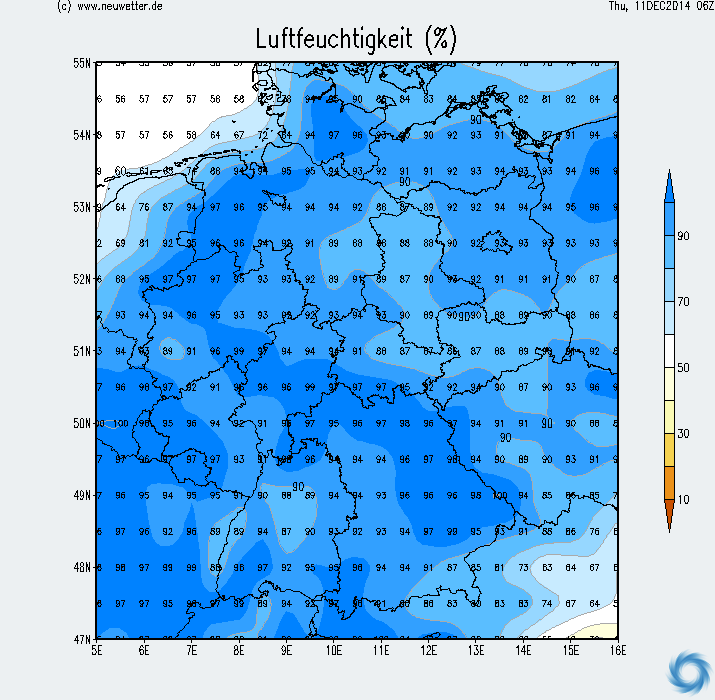
\includegraphics[width=\textwidth]{feuchtigkeit}
\end{figure}

\section{Sensorknoten}

Sensorknoten gibt es natürlich in verschiedenen Formen und Größen, doch gewisse Grundelemente sind in jedem Sensorknoten gleich. In Abbildung \ref{fig:sensornode} ist ein grober Aufbau beschrieben. In der heutigen Zeit befinden sich dabei alle Bauteile auf einem einzigen Chip, man spricht daher von einem System-on-a-Chip.\newline
Natürlich ist das wohl charakteristischste Bauteil, denn es macht einen Netzwerkknoten zum Sensorknoten, ein Sensor. Es ist ebenso möglich, dass ein Sensorknoten viele verschiedene Sensoren besitzt, um an der Position mehrere verschiedene Parameter aufnehmen zu können.\newline
Um aber mit den Messwerten etwas anfangen zu können, sind auch andere Bauteile essentiell. 

\begin{itemize}
\item Ein Prozessor, typischer Weise auf einem Mikrocontroller, muss sich dabei um die Steuerung der anderen Bauteile kümmern.
\item Ein Funkmodul ermöglicht dem Knoten die Kommunikation mit Anderen in seiner erreichbaren Umgebung. Nur dadurch ist es möglich in großflächigen Netzwerken die Daten auswerten zu können, da es in manchen Gebieten sogar unmöglich sein kann, die Knoten nach dem verstreuen noch direkt zu erreichen.
\item Ein Speicher sollte ebenfalls auf einem Knoten vorhanden sein. Zum einen müssen natürlich Programme, die der Prozessor ausführt gespeichert werden. Ebenso ist es denkbar, dass die Funkkommunikation gelegentlich für längere Zeit abgeschaltet wird, um so Energie zu sparen. Wenn innerhalb dieses Zeitraums relevante Messwerte bestimmt wurden, so sollen diese natürlich nicht einfach verfallen, sondern bis zur nächsten Funkverbindung gesichert werden.
\item Irgend eine Art von Energiequelle ist auch für einen Sensorknoten entscheidend, um funktionieren zu können. Dazu gehört typischer Weise eine Batterie. Weiterhin ist es denkbar, durch energy harvesting zusätzlich Energie zu gewinnen. Da dies aber nicht unbedingt rund um die Uhr möglich ist, muss auch in diesem Fall die gewonnene Energie zunächst gespeichert werden.
\end{itemize}

\begin{figure}[htbp]
\centering
\caption{Sensorknoten}
\label{fig:sensornode}
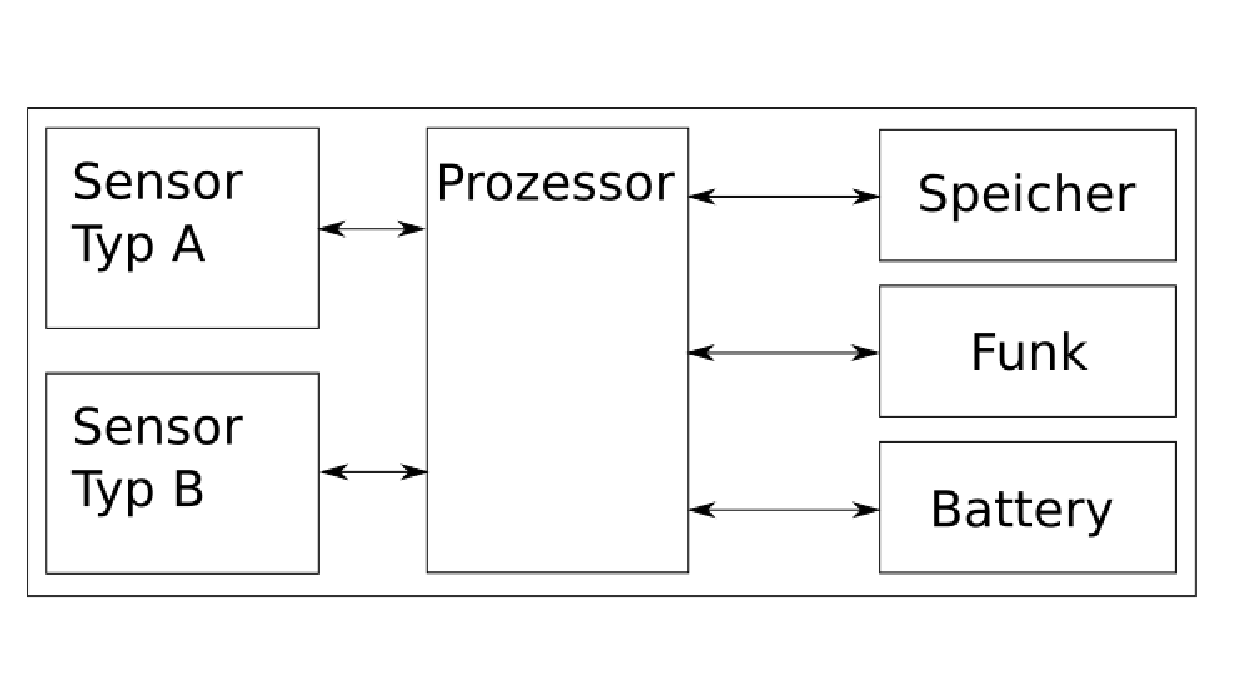
\includegraphics[width=\textwidth]{SensorNode}
\end{figure}

\section{Sensornetzwerke}

Da ein einzelner Sensorknoten nur sehr begrenzt einsetzbar ist, werden die immer kleiner und mobiler werdenden Knoten oft zu großen Netzwerken verbunden. Dadurch ist es möglich große Flächen mit den Messwerkzeugen abzudecken. So ist es möglich detaillierte Daten von einem Gebieten zu erhalten.\newline
Bei einem sehr großen Netzwerk ist ein gutes Routing sehr wichtig, besonders da die Knoten sehr abhängig von der effizienten Nutzung der Energiequelle sind. Für das Übertragungsprotokoll kommt dabei meist der Standard IEEE 802.15.4 zum Einsatz, da dieser für Drahtlose Kommunikation mit niedriger Übertragungsrate und für Geräte mit geringer Leistungsaufnahme ausgelegt ist. Es deckt lediglich die unteren beiden Schichten des OSI-Modells ab.\newline
Die Verbindung zu Anwendungsschicht stellt dann beispielsweise das ZigBee-Framework dar. 
	%\chapter{Anforderungen}

	\chapter{Simulationsumgebung}

Um eine Simulation in einem geeigneten zeitlichen Rahmen erstellen zu können, bietet sich die Verwendung von einer Simulationsumgebung an. Diese enthält hauptsächlich ein Framework mit vielen Bibliotheken, welche für den speziellen Anwendungsfall viel Arbeit ersparen können. \newline
Es gibt eine große Auswahl an verschiedenen Simulationsumgebungen, wobei jede ihre Vor- und Nachteile mit sich bringt. Wichtig für die Arbeit ist ein Simulator der Netzwerke bereitstellt und auch drahtlose Kommunikation ermöglicht. Es sollten eigene Knoten erstellt und angepasst werden können, damit die Hardwaresensorik und das Verhalten im Umgang mit Nachrichten untereinander genau definiert werden können. Auch Funktionen für die Repräsentation von Batterieeigenschaften und die Erfassung und Analyse von Statistiken sollten vorhanden sein.\newline
Im Falle von speziellen Anforderungen der Frameworks sollte eine IDE vorhanden sein, die diese unterstützt. Auch eine sehr wichtige Anforderung an den Simulator ist eine grafische Umgebung für die Simulation selbst, sodass Informationen nicht nur aus Dateien ausgelesen werden können, sondern für den Nutzer auch auf den ersten Blick sichtbar sind.

\section{wichtige Simulationsumgebungen}

Es gibt viele Umgebungen zum Simulieren von Netzwerken. Zunächst werden hier 4 Wichtige vorgestellt: die \textbf{IKR Simulation Library (IKR SimLib)} von der Universität Stuttgart, der \textbf{Open Source Wireless Network Simulator} kurz \textbf{openWNS} von der Universität Aachen, \textbf{ns-3} vom ns-3 project und \textbf{Simanet} von der TU Chemnitz.

\paragraph{Simulation Library (IKR SimLib)\cite{ikr}}

Eine freie Simulationsbibliothek unter der Lizenz GNU LGPL für Kommunikationsnetzwerke in C++ und Java von der Universität Stuttgart. Diese steht für Linux und Unix(-artige) Systeme zur Verfügung, während die Verwendung unter Windows nicht offiziell getestet wurde.\newline
Da es lediglich eine Bibliothek für Java darstellt, existieren keine extra IDE und auch keinerlei GUI oder ähnliche Hilfswerkzeuge. Allerdings kann ein Projekt mit jeder normalen Java- oder C++ IDE benutzt werden, schließlich muss nur die Bibliothek importiert werden.\newline
Da schon seit den 1980ern an IKR SimLib entwickelt wird, kann die Bibliothek weitreichende Funktionalitäten zur Verfügung stellen, wie zum Beispiel Unterstützung für mobile, IP- oder P2P-Netzwerke.

\paragraph{openWNS\cite{openwns}}

OpenWNS ist ein Simulator für kabellose Kommunikation, entwickelt von der Universität Aachen. Das Projekt steht kostenlos zur Nutzung bereit und ist mit der LGPLv2 lizensiert. \newline
Es wurde speziell für Linux entwickelt, es läuft allerdings auch unter Windows. Die Entwicklung erfolgt in Python. Für grafische Unterstützung sorgt das integrierte Tool Wrowser\cite{wrowser}, welches in erster Linie dazu dient die Resultate der Simulation zu sammeln und die Messwerte zu visualisieren, aber auch beim Erstellen einer Simulation Hilfestellungen bietet, wie beispielsweise beim Einrichten der Simulationsdatenbank.\newline
Es gibt keine extra für openWNS erstellte oder angepasste IDE, allerdings wird in der Dokumentation beschrieben, wie der Texteditor Emacs\cite{emacs} den speziellen Anforderungen vom openWNS-Stil angepasst werden kann. Allerdings ist es notwendig für die Entwicklung stets einen Texteditor, den Wrowser und die Kommandozeile zu benutzen, was im Vergleich zu einer alles umfassenden IDE deutlich weniger komfortabel ist.

\paragraph{NS-3\cite{ns3}}

ns-3 ist ein freier Netzwerksimulator, der unter der GPLv2 lizensiert ist. Das Erstellen der Simulationen funktioniert mithilfe der Sprache Python. Dafür steht keine extra IDE zur Verfügung, was allerdings auch nicht notwenig ist, da es genügend andere Python-Umgebungen gibt.\newline
Es werden sowohl kabelgebundene als auch kabellose Verbindungen unterstützt. Allerdings besteht nicht für alle wichtigen Protokolle eine Unterstützung, wie beispielsweise WSN.\newline
Ein weiterer großer Nachteil ist, dass es keine Oberfläche während der Ausführung gibt. Die Simulation wird per Textausgabe auf der Kommandozeile ausgeführt. Die gesammelten Daten können anschließend mit Plot-Tools visualisiert werden. Für das Generieren von Netzwerken steht jedoch ein grafisches Hilfsmittel zur Verfügung. Mit dem Topology Generator\cite{TopGen} können per GUI Netzwerke angelegt werden und anschließend in C++ oder Python-Code umgewandelt werden. 

\paragraph{Simanet\cite{simanet}}

Simanet ist ein Projekt, welches an der TU Chemnitz entstanden ist. Es eignet sich sehr gut für das Simulieren von Funkkommunikation und daher zum Testen von Routingverfahren.\\
Im Vergleich zu anderen Simulatoren wie Omnet++ oder ns-3 ist Simanet sehr leichtgewichtig und eignet sich daher hervorragend für sehr große Simulationen.\\
Es gibt zahlreiche vorhandene Module, die wichtige Funkstandards wie WLAN oder ZigBee, Energiemodelle, Lokalisierung und auch Visualisierung und Auswertung abdecken.

\paragraph{Omnet++\cite{omnet}}

Omnet++ ist ein Framework für die Simulation von Netzwerken, welches unter der ACADEMIC PUBLIC LICENSE steht. Die Nutzung ist daher kostenfrei und der Quellcode ist offen und darf verändert werden.\\
Es bietet eine angepasste IDE, welche die Besonderheiten der NED-Sprache und auch den C++-Code interpretieren kann.\\Die Simulation selbst bietet ein grafisches Interface und auch für die Auswertung von statistischen Daten stehen grafische Hilfsmittel innerhalb der IDE bereit.\\
Der größte Vorteil von Omnet++ ist die Möglichkeit, Code auf dem Application Layer der Sensorknoten ausführen zu können, was bei vielen andern Simulatoren nicht möglich ist.\\
Funkkommunikation ist standardmäßig in Omnet++ zwar nicht möglich, aber durch das MiXiM-Framework wird diese implementiert.

\paragraph{weitere}

Es gibt natürlich außer den bisher genannten Simulationsumgebungen auch noch weitere, auf die hier aber nicht näher eingegangen werden soll. So gibt es beispielsweise GloMoSim, welches die parallele Programmiersprache Parsec benutzt. Es ist geeignet um sowohl kabellose, als auch -gebundene Netzwerke zu simulieren, jedoch wird es zum aktuellen Stand nicht mehr weiterentwickelt. \newline
Eine weitere Alternative wäre NetSim, welches von Tetcos, zusammen mit dem Indian Institute of Science entwickelt wurde. Die bestehenden Bibliotheken sind in C geschrieben und implementieren viele Protokolle wie beispielsweise WLAN, TCP oder LTE.

\section{Vergleich}

Simanet unterstützt leider keine komplexe Codeausführung innerhalb von Netzwerkknoten. Es ist daher für diese Arbeit nicht geeignet, da das Verhalten der Sensorik nicht abgebildet werden kann. Daher wird Simanet im folgenden Vergleich nicht weiter berücksichtigt. 

\begin{table}[!ht]
  \centering
  \caption{Übersicht Simulatoren}
  \label{Übersicht Simulatoren}
\begin{tabularx}{\textwidth}{lllll}
	\toprule
	& Omnet++ & IKR SimLib & OpenWNS & NS-3 \\
	\midrule
	\specialcell{freie Lizenz}  & \cmark & \cmark(LGPL) & \cmark (LGPLv2) & \cmark (GPLv2) \\
	\specialcell{alle gängigen\\Betriebssysteme} & \cmark & \specialcell{kein\\Windows} & \cmark & \specialcell{kein\\Windows} \\
	\specialcell{GUI bei Simulation} & \cmark & \xmark & (\cmark) & \xmark \\
	IDE & \cmark & (\xmark) & (\xmark) & (\cmark) \\
	Drahtlose Verb. & (\cmark) mit MiXiM & \cmark & \cmark & \cmark \\
	Sprache(n) & C++ mit NED & C++ oder Java & Python & Python \\
	\bottomrule
\end{tabularx}
\end{table}

In Tabelle \ref{Übersicht Simulatoren} ist ein direkter Vergleich der größten Unterschiede zwischen den Simulatoren Omnet++, IKR SimLib, OpenWNS und NS-3 aufgezeigt. Es ist sehr positiv zu bewerten, dass alle Simulationsumgebungen über freie Lizenzen verfügen und die für die Arbeit relevante drahtlose Kommunikation ermöglichen.\newline
Der größte Nachteil der Simulatoren IKR SimLib und ns-Simulator liegt darin, dass beide keine grafische Umgebung für die Simulation selbst bieten. Das wirkt sich wiederum natürlich positiv auf die Performanz aus, allerdings lässt sich über eine grafische Übersicht deutlich leichter und schneller ein Eindruck über die Zustände der Simulation gewinnen. Ein weiterer Nachteil der beiden ist die eingeschränkte Verfügbarkeit auf verschiedenen Betriebssystemen. \newline
OpenWNS bietet nur teilweise Unterstützung in grafischer Hinsicht. Es ist möglich mithilfe des sogenannten Wrowser die Simulation zu starten und die statistischen Daten zu erfassen. Jedoch bietet es keine so umfassende Oberfläche wie Omnet++. \newline
Letztendlich ist die Entscheidung zugunsten von Omnet++ gefallen. Die Simulationsumgebung wird im folgenden Abschnitt ausführlicher beschrieben.

\section{Omnet++}

\subsection{Einleitung}

Omnet++\cite{omnet} ist eine C++-Bibliothek und ein C++-Framework, welches primär zum Simulieren von Netzwerken dient. Außerdem bietet es eine Netzwerkbeschreibungssprache namens NED (NEtwork Description) und eine auf Eclipse\cite{eclipse} basierende Entwicklungsumgebung. Für die Simulation besteht außerdem ein grafisches Interface, mit dem die Kommunikation der Knoten im Netzwerk gut verfolgt werden kann.
\newline Standardmäßig werden keine mobilen oder kabellosen Protokolle in Omnet++ unterstützt. Jedoch kann mithilfe des MiXiM-Frameworks die Funktionalität um eben diese erweitert werden.
\newline Es bietet unterstützt alle gängigen Betriebssysteme wie Linux, andere unixbasierte Systeme, Mac OS und Windows und besitzt außerdem eine kostenlose Lizenz.

\begin{figure}[htbp]
\centering
\caption{GUI bei der Ausführung einer Simulation }
\label{fig:messageEvent}
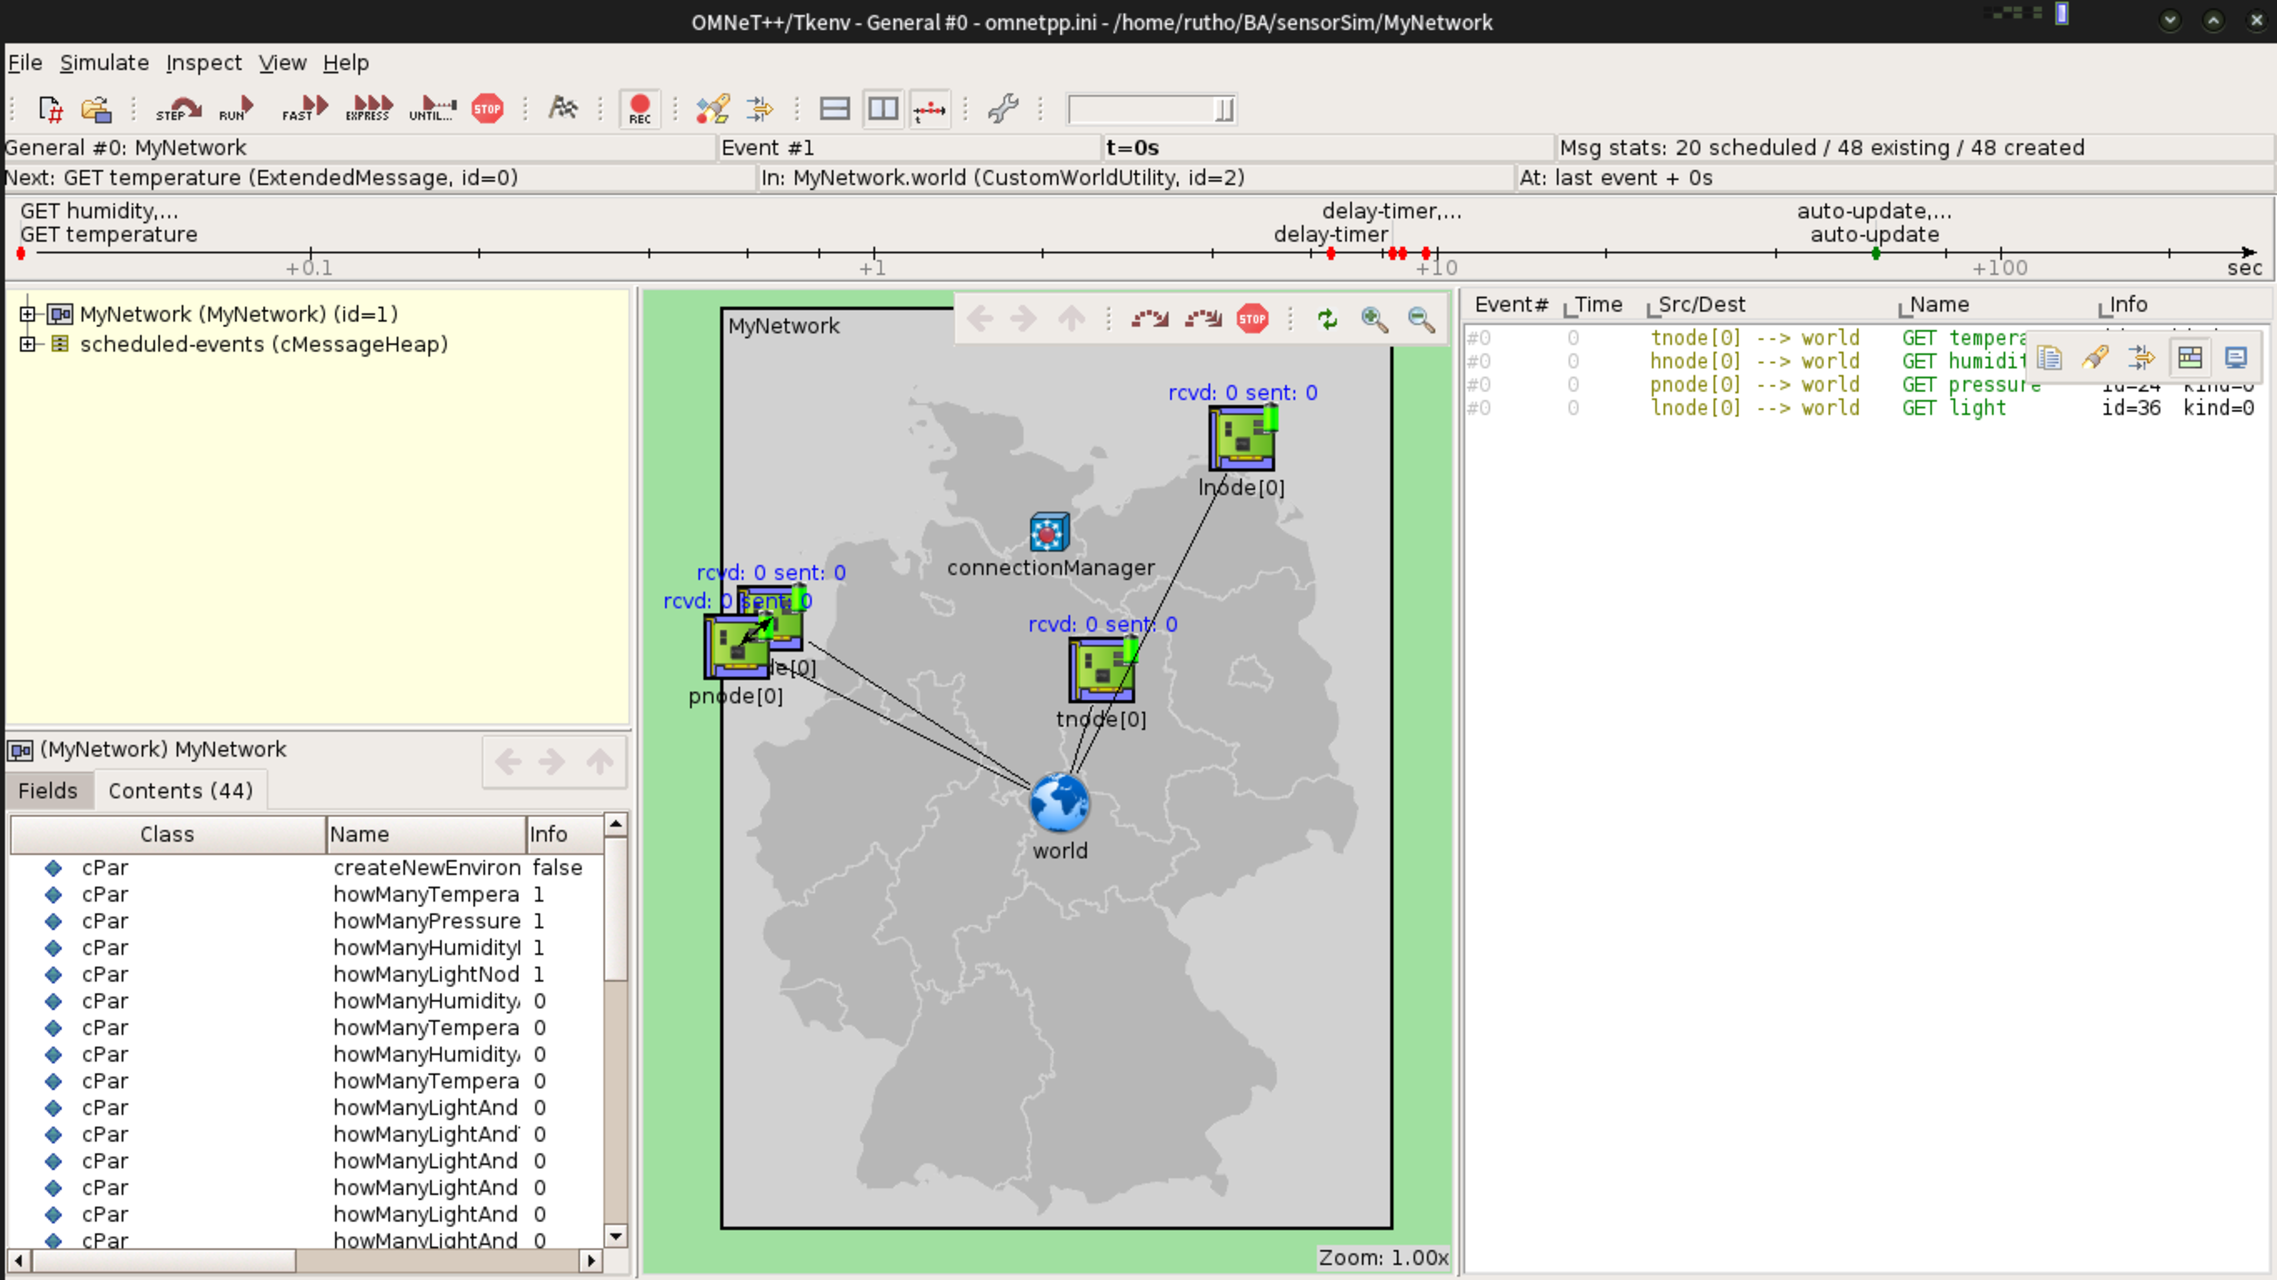
\includegraphics[width=\textwidth]{SimulationUI}
\end{figure}

\subsection{NED language}

Die Netzwerkbeschreibungssprache NED\cite{ned} bietet eine Möglichkeit, auch komplexe Netzwerke relativ einfach zu beschreiben und darzustellen. Man kann schnell ein einfaches Modul mit Gates (siehe Listing \ref{lst:simpleNode}) für die Kommunikation beschreiben oder ihm Submodule für verschiedene andere Aufgaben zuweisen und dieses in ein Netzwerk integrieren und dort mehrere und auch verschiedene Instanzen von Modulen verknüpfen (siehe Listing \ref{lst:simpleNetwork}).
\newline
Dabei helfen die verschiedenen möglichen Module. Es können die 3 Typen simple, module und network definiert werden. Wie der Name schon sagt, ist network dazu da ein Netzwerk zu beschreiben und sollte alle nötigen Module als Submodule beinhalten. 
\newline
Mit dem Schlüsselwort module lassen sich komplexe Objekte beschreiben. Neben den Standardvariablen wie beispielsweise Parameter, Gates oder Connections lassen sich auch Submodule definieren. Dadurch ist es möglich verschiedene in sich abgeschlossene Modulteile in einem großen Modul zu vereinen.
\newline
Geeignet als ein solches Modulteil ist wiederum das simple-Modul. Dieses kann keine weiteren Submodule besitzen, sondern lediglich einfache Funktionalität definieren.\\
Wenn nicht anders über den Parameter @class angegeben sucht \textbf{Omnet++} nach einer Klasse, die den gleichen Namen wie das erstellte Modul besitzt. In dieser können Funktionen deklariert und implementiert werden, die das Verhalten des Moduls beeinflusst. Welche Funktionen von \textbf{Omnet++} interpretiert werden, wird im Kapitel \ref{para:Nodes and Messages} näher erklärt.
Eine Übersicht mit Kurzbeschreibung zu den wichtigsten Schlüsselwörtern in NED in der Tabelle \ref{tab:NED} zu finden.

\begin{table}[!ht]
  \centering
  \caption{NED Schlüsselbegriffe}
\begin{tabularx}{\textwidth}{lll}
	\toprule
	Kategorie & Begriffe & Funktion \\
	\midrule
	\multirow{6}{*}{Modulart} & network & ein Netzwerk, 1 pro Simulation\\
	& simple & ein einfaches, eigenständiges Modul\\
	& module & ein compound Modul, kann Submodule haben\\
	& channel & beschreibt eine Verbindung zwischen Gates\\
	& channelinterface & ein Interface für Channel\\
	& moduleinterface & ein Interface für Module\\
	\midrule
	\multirow{5}{*}{\specialcell{Sections\\von\\Modulen}} & types & um eigene Typen im Modul zu definieren\\
	& parameters & Parameter des Moduls definieren\\
	& submodules & andere Module integrieren\\
	& gates & Schnittstellen für Kommunikation definieren\\
	& connections & Gates miteinander verbinden\\
	\midrule
	\multirow{3}{*}{Typen} & \multicolumn{2}{l}{int, string, double, bool}\\
	& xmldoc & speichert den Pfad eines XML-Files\\
	& xml	 & speichert XML\\
	\midrule
	\multirow{5}{*}{Verbindungen} & allowunconnected & \specialcell{erlaubt Kommunikation zwischen Gates \\ohne definierte Verbindung}\\
	& input & definiert ein Gate als eingehend\\
	& output & definiert ein Gate als ausgehend\\
	& inout & legt je ein in- und output Gate an\\
	\midrule
	\multirow{7}{*}{weitere} & @display & Eigenschaften zur Darstellung bei Sim.\\
	& @class & spezielle C++-Klasse zum Modul definieren \\
	&package & definiert den Namensraum\\	
	& import & andere Pakete und Module einbinden\\
	&\multicolumn{2}{l}{volatile, const, extends,import,like}\\
	&\multicolumn{2}{l}{this,false,true,default, if,and,or,else,for}\\
	&\multicolumn{2}{l}{index,sizeof,typename}\\
	\bottomrule
\end{tabularx}
\label{tab:NED}
\end{table}

\begin{figure}[htbp]
\centering
\caption{Oberfläche der Entwicklungsumgebung mit Bespiel für die NED-Integration}
\label{fig:messageEvent}
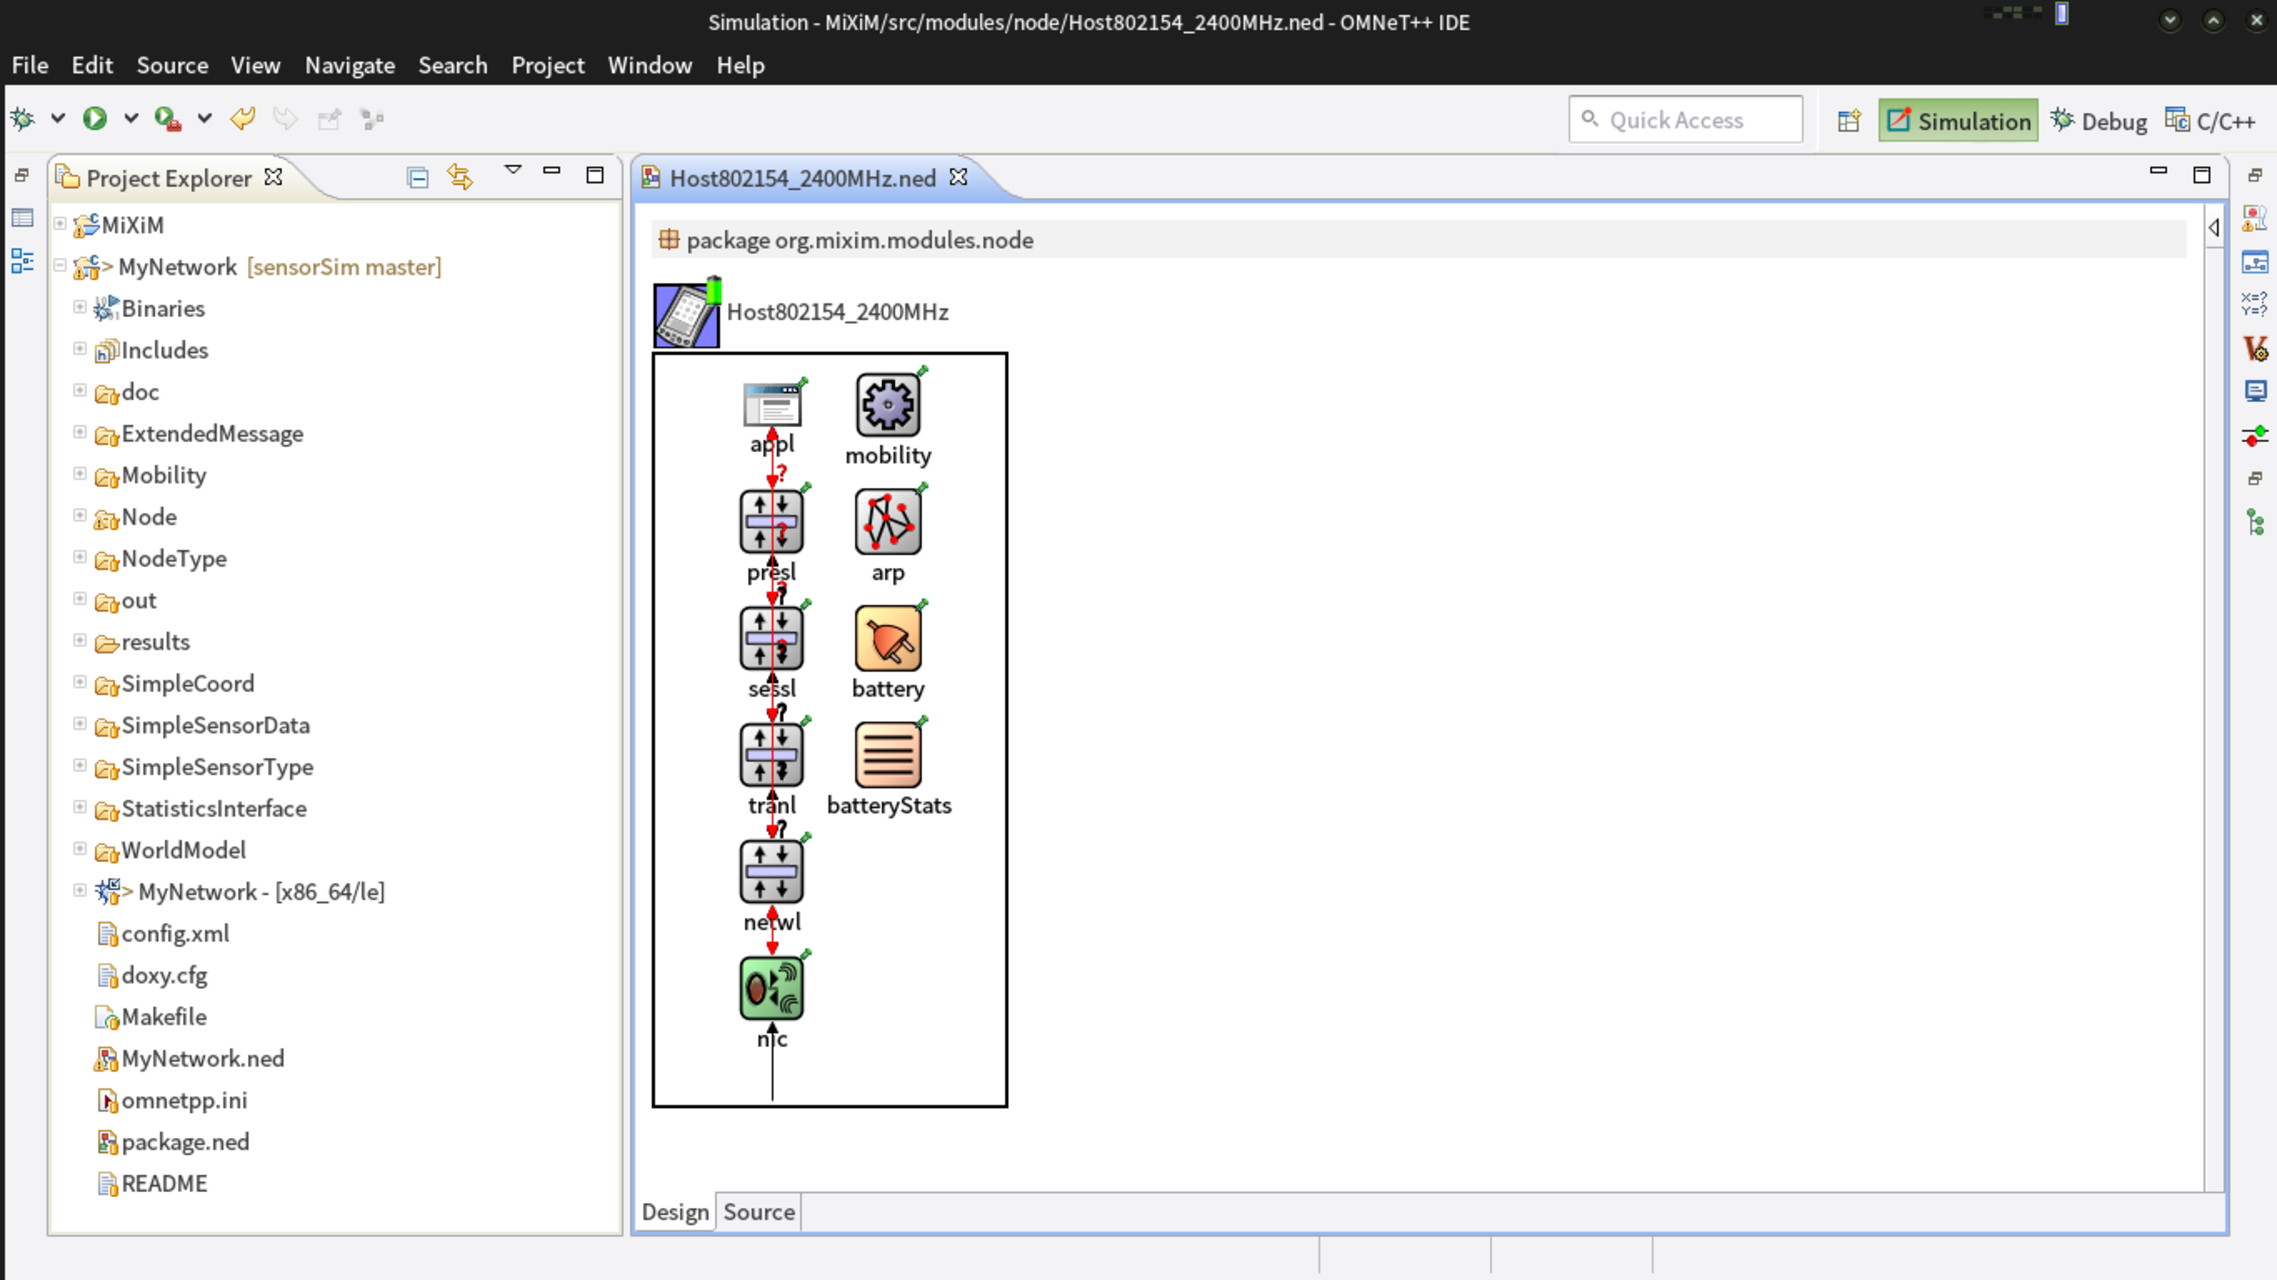
\includegraphics[width=\textwidth]{omnetEclipse}
\end{figure}

\paragraph{Beispiel} Ein kurzes Beispiel soll das Zusammenspiel einiger wichtiger Schlüsselworte aufzeigen:

Zunächst wird ein einfach Modul (Listing \ref{lst:simpleNodeLed}) erstellt, welches eine LED repräsentiert. Dieses erhält dafür einen Parameter vom Typ boolean, welcher anzeigt, ob die LED leuchtet und einen eingehenden Port, welcher die Lampe steuern kann. 
\begin{lstlisting}[language=ned,caption={einfaches Modul: LED},label=lst:simpleNodeLed]
simple LED
{
	parameters:
		bool ledLeuchtet;
	gates:
		input control;
}
\end{lstlisting}

Als zweites Modul, ebenso wie die LED vom Typ simple, wird ein einfach Knopf (Listing \ref{lst:simpleNodeButton}) definiert. Dieser hat ein input-Gate über welches einen Knopfdruck simulieren kann und ein ausgehendes Gate, welches im Falle eines Knopfdrucks ein Signal ausgeben kann.
\begin{lstlisting}[language=ned,caption={einfaches Modul: Knopf},label=lst:simpleNodeButton]
simple Knopf
{
	gates:
		input buttonStateChange;
		output signal;
}
\end{lstlisting}

Als drittes wird ein Modul vom Typ module definiert (Listing \ref{lst:simpleNode}). Es handelt sich dabei um ein Compound-Modul. Dieses kann genutzt werden, um verschiedene simple-Module auf sich zu vereinen und die Interaktion zwischen diesen zu ermöglichen. So können komplexe Bauteile modular definiert werden.\\
Das Modul repräsentiert einen Bauteil, welches einen Knopf und eine LED besitzt. Zusätzlich besitzt es ein eingehendes und ein ausgehendes Gate. Das output-Gate vom Knopf ist mit dem eingehendes Gate von der LED verbunden, den durch einen Knopfdruck soll die LED ein- oder ausgeschaltet werden können.
\begin{lstlisting}[language=ned,caption={Compound Modul},label=lst:simpleNode]
module Knoten
{
	parameters:
		string name="KnotenMitLedUndKnopf";
	submodules:
		Blinker: LED {
		}
		Button: Knopf {
		}
	gates:
		input in;
		output out;
	connections:
		Button.signal --> Blinker.control;
}
\end{lstlisting}

Da es sich in Omnet++ um eine Netzwerksimulation handelt, wird einschließend noch ein kleines Netzwerk aus den vorher definierten Modulen aufgebaut werden (Listing \ref{lst:simpleNetwork}). Dabei werden zwei Module vom Typ Knoten erstellt und die jweiligen Gates der Beiden miteinander verbunden.
\begin{lstlisting}[language=ned,caption={einfaches Netzwerk},label=lst:simpleNetwork]
network Netzwerk
{
	submodules:
		node1: Knoten;
		node2: Knoten;
	connections:
		node1.in <-- node2.out;
		node1.out --> node2.in;
}
\end{lstlisting}

\subsection{Einige Techniken, Funktionen und wichtige Module}

Im folgenden Abschnitt wird ein Ausschnitt darüber gegeben, was Omnet++ an Funktionalitäten bereitstellt. Grundlegend wird für eine einfache Simulation ein Netzwerk benötigt, welches in der Netzwerkbeschreibungssprache NED beschrieben wird. Dieses Netzwerk kann dann Nodes definieren, welche selbst Module sind, welche wiederum auch in NED beschrieben werden. Wenn diese Module ausgehende und/oder eingehende Gates besitzen, können diese im Netzwerk wiederum miteinander verbunden werden.\newline
Dieser einfache Grundaufbau genügt im Prinzip schon, damit eine valide Simulation ablaufen kann. Um dazu noch etwas Funktionalität in die Module zu bringen ist es möglich, für jedes Modul eine Klasse in C++ zu definieren. Man kann zum einen eigene Klassen definieren oder die in der Simulationsbibliothek vorhandenen Klassen nutzen.\newline
Zusätzlich zur Standardbibliothek gibt es noch 3 relevante Frameworks, die weitere Funktionen zur Verfügung stellen: MiXiM, INET und Castalia.

\subsubsection{Nodes and Messages}\label{para:Nodes and Messages}

Für die Steuerung innerhalb einer Simulation sind Nachrichten das wichtigste Werkzeug in \textbf{Omnet++}. So kann man eine Nachricht zu einer festgelegten Simulationszeit verschicken, um diese als Events einzusetzen. Dabei können Knoten auch Nachrichten an sich selbst versenden.

Um einem selbst definierten Modul die Möglichkeit zu geben Nachrichten zu verstehen und zu benutzen werden einige Funktionen bereitgestellt, die man selbst definieren muss.

Diese sind für die Funktionalität eines \textbf{cSimpleModule} entscheidend und sollten nach dem Erstellen eines neuen Moduls implementiert werden:

\begin{itemize}
\item void initialize()
\item void handleMessage(cMessage *msg)
\item void activity()
\item void finish()
\end{itemize}

\paragraph{initialize()}

Die Funktion \textbf{initialize()} wird nach dem Erstellen eines Moduls aufgerufen. Es kann so ähnlich wie ein Konstruktor verwendet werden. Entscheidend ist, dass die Methode erst aufgerufen wird, nachdem auch der \textbf{NED}-Teil des Moduls eingelesen wurde. Das bedeutet, dass erst an dieser Stelle auf Parameter des Moduls zugegriffen werden kann und das ist im Konstruktor noch nicht möglich. Auch Nachrichten kann das Modul erst ab diesem Zeitpunkt verschicken.

\paragraph{handleMessage(cMessage *msg)}

Diese Methode kann eingehende Nachrichten auswerten. Sollten bei einem Modul Nachrichten ankommen, ohne dass diese Funktion definiert wurde, wird ein Fehler auftreten. Wie Nachrichten genauer aufgebaut sind, ist im Abschnitt \textbf{cMessage} beschrieben.
Nachrichten können zeitgesteuert Events auslösen. Die Methode \textbf{handleMessage()} ist somit das Herzstück der meisten Module, da hier das komplette Verhalten geregelt wird. \newline
Es können im Regelfall natürlich viele verschiedene Arten von Nachrichten in einem Modul eintreffen, die auch unterschiedlich behandelt werden müssen. Zur Fallunterscheidung stehen wiederum viele Funktion im Nachrichtenmodul zur Verfügung, die beispielsweise Informationen über den Sender liefer, ob die Nachricht eine Selfmessage war, also vom Modul an sich selbst gesendet wurde oder einfache Informationen wie der Name der Nachricht.

\paragraph{activity()}

Diese Methode ist eine eher unwichtige Funktion. Wenn \textbf{handleMessage()} korrekt verwendet wird, sollte man auf die Benutzung von \textbf{activity()} am besten komplett verzichten. Es verhält sich oberflächlich betrachtet wie \textbf{handleMessage()}, allerdings wird diese Methode nicht einfach aufgerufen, sollte eine Nachricht ankommen, sondern läuft in einer Endlosschleife und wartet Permanet aktiv auf Nachrichten. Daher ist sie wesentlich rechenintensiver als das Gegenstück \textbf{handleMessage()}.

\paragraph{finish()}

Diese Methode wird aufgerufen, nachdem die Simulation beendet wurde und noch bevor das Modul gelöscht wurde. Sie sollte nicht zum Löschen anderer Module verwendet werden, da nach dem Aufruf von finish() die Simulation erneut gestartet werden kann, ohne dass das Netzwerk komplett neu initialisiert wird. Wenn allerdings wichtige Module an dieser Stelle gelöscht wurden, ist ein Neustart nicht mehr möglich.\newline
Die Methode ist stattdessen dafür da die eben abgelaufene Simulation auszuwerten. Es können an dieser Stelle alle relevanten Informationen gespeichert werden, damit diese hinterher statistisch ausgewertet werden können.

\subsubsection{cMessage}

Für die Nachrichten selbst existiert ein fertig implementiertes Modul namens \textbf{cMessage}. Dieses erfüllt schon die wichtigsten Anforderungen, die man an ein Nachrichtenmodul stellt. So können Nachrichten nicht nur \textbf{strings} übertragen, sondern alle Klassen, die von \textbf{cNamedObject} erben. Man kann also auch komplexe, selbst definierte Objekte mithilfe von cMessage übertragen.\\
Es empfiehlt sich dennoch eine eigene Kindklasse von cMessage zu definieren, da man in diesem eigene Parameter definieren kann, die verschiedene Werte beschreiben. So kann man zum Beispiel genauere Informationen für Quelle und Senke in der Nachricht speichern oder verschiedene Werte für Statistiken. Sollte man eine veränderte Kindklasse von cMessage definieren, so wird zusätzlich eine Klasse dazu generiert, die viele Funktionen bereitstellt, die zum Beispiel das Kopieren einer Nachricht ermöglichen - auch inklusive der extra hinzugefügten Parameter.

\begin{table}[!ht]
  \centering
  \caption{Übersicht über einige Funktionen von cMessage}
\begin{tabularx}{\textwidth}{rll}
	\toprule
	typ & Funktion & Kurzbeschreibung\\
	\midrule	
	virtual cArray \& & getParList () & Parameterliste einer Nachricht\\
	bool 	& isSelfMessage () const & ist Nachricht an sich selbst\\
	cModule * 	& getSenderModule () const & \multirow{4}{*}{\specialcell{Informationen über Sender\\äquivalent für Arrival vorhanden}} \\
	cGate * 	& getSenderGate () const  & \\
	int &	getSenderModuleId () const & \\
	int &	getSenderGateId () const & \\
	simtime\_t\_cref 	& getCreationTime () const & Zeitpunkt: Nachricht erstellt\\
	simtime\_t\_cref 	& getSendingTime () const & Zeitpunkt: Nachricht gesendet\\
	simtime\_t\_cref 	& getArrivalTime () const  & Zeitpunkt: Nachricht angekommen\\
	bool &	arrivedOn (int gateId) const & Id des Inputgate\\
	\bottomrule
\end{tabularx}
\end{table}

\subsubsection{XML Support}

NED-Parameter eines Moduls können vom Typ xml sein. Die dazu gehörende Klasse cXMLElement bietet ihrerseits umfangreiche Unterstützung dafür an. Diese orientiert sich dabei an einem DOM-Parser, ist allerdings aus Performanzgründen nur ähnlich aufgebaut. Dabei stellt die Klasse die für X-Path typischen Funktionen für XML-Zugriffe bereit wie zum Beispiel \textbf{getParentNode()} oder \textbf{getChildren()}.

\begin{minipage}{\textwidth}
\begin{lstlisting}[language=C++,caption={Beispiel einlesen von XML},label=lst:xml]
cXMLElement *rootE = par("xmlFile").xmlValue();
cXMLElementList nListRows = rootE->getChildren();
int amountRows = nListRows.size();
int* data = new int[amountRows];
for (int i = 0; i < amountRows; i++){
    //nListRowArray ist eine Zeile aus dem XML file 
    //bzw. alle Elemente 1. Ebene unter der Wurzel
    cXMLElement* nListRowArray = nListRows[i];
    //kann ab hier beliebig tief fortgesetzt werden
}
\end{lstlisting}
\end{minipage}

\subsubsection{Statistiken}

Um die durchgeführten Simulationen ordentlich auswerten zu können, stellt Omnet++ verschiedene Werkzeuge bereit. Neben dem Eventlog ist es möglich, während der Simulation Skalar- sowie Vektorwerte zu definieren. Die Skalarwerte besitzen dabei einen fixen Wert, wogegen Vektoren die Veränderung von bestimmten Variablen im Laufe der Simulationszeit speichern können. Die dazugehörigen Klassen heißen cLongHistogram und cOutVector.\\
Diese beiden Werte können nach dem erfolgreichen Abschließen einer Simulation auch grafisch ausgewertet werden. Dazu kann nach dem Exportieren der Werte in der Simulationsumgebung ausgewählt werden, welche Daten zusammen in einem Diagramm dargestellt werden sollen. Zum Erstellen der Graphen wird Gnuplot\cite{gnuplot} genutzt. Anschließend können noch verschiedene Einstellungen getroffen werden, damit die Daten möglichst gut visualisiert werden können. Beispielsweise kann der Typ des Kurvenverlaufs gewählt werden. In den Bildern \ref{fig:statRight} und \ref{fig:statWrong} ist ein Beispiel dafür. Es liegt ein Automat vor, welcher zwischen 3 Zuständen wechselt. Dabei zeigt\ref{fig:statRight} die wesentlich besser Variante des Graphen.

\begin{figure}[htbp]
\centering
\caption{Zustandswechsel Automat falsch}
\label{fig:statWrong}
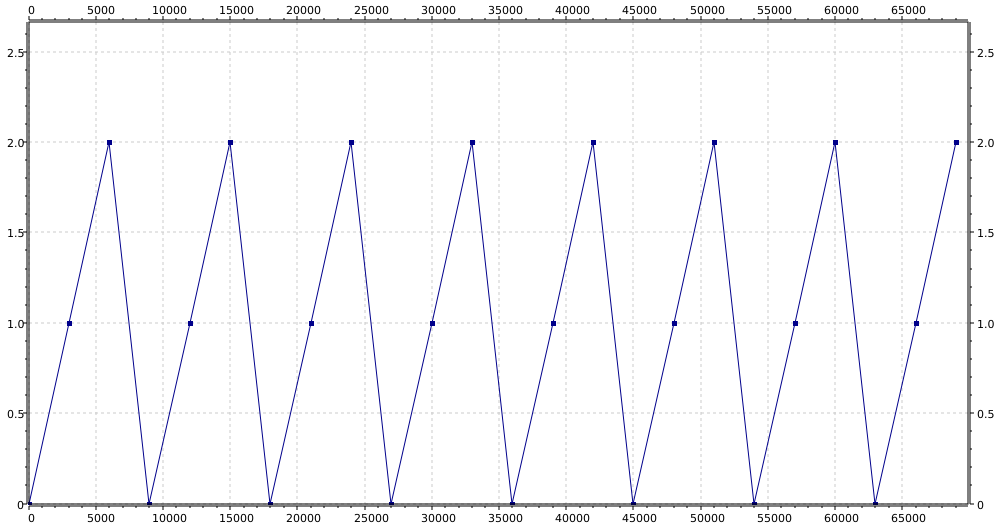
\includegraphics[width=\textwidth]{statWrong}
\end{figure}

\begin{figure}[htbp]
\centering
\caption{Zustandswechsel Automat richtig}
\label{fig:statRight}
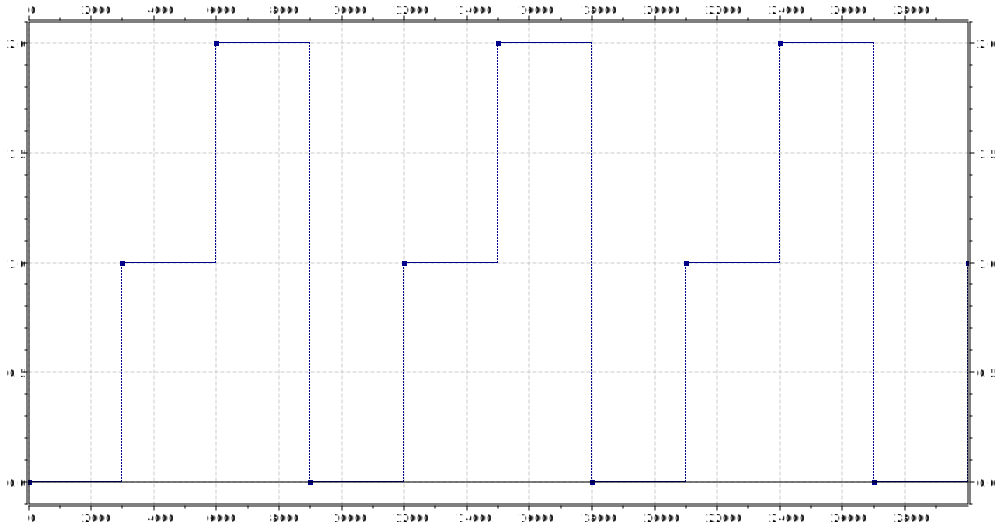
\includegraphics[width=\textwidth]{statRight}
\end{figure}

\subsubsection{weitere Beispiele}

\paragraph{cClassDescriptor} Eine Klasse, die dabei behilflich ist, die Felder eines Objektes zu finden. Dazu muss eine Klasse lediglich von cClassDescriptor erben. Die Verwendung funktioniert wie im Listing \ref{lst:cclassdescriptor} beschrieben. 

\begin{minipage}{\textwidth}
\begin{lstlisting}[language=C++,caption={Verwendung von cClassDescriptor },label=lst:cclassdescriptor]
cClassDescriptor* thisDescr = cClassDescriptor::getDescriptorFor(this);
int count = thisDescr->getFieldCount(this);

for ( int i = 0; i < count; i++) {
    std::stringstream s;
    s << i <<" " << thisDescr->getFieldName(this, i) << " " ;
    s << thisDescr->getFieldAsString(this, i, 0);
    s << i << " " << thisDescr->getFieldName(this, i);
    cMessage *msg = new cMessage(s.str().c_str());
    send(msg, "gate$o");
}
\end{lstlisting}
\end{minipage}

\paragraph{Simulationszeit und Events}

Die Zeit einer Simulation verläuft linear. Anhand dieser kann die Ausführung von Events für einen bestimmten Zeitpunkt geplant werden. Dies ist möglich durch das Versenden von cMessage in Kombination mit einer Scheduletime und wenn nötig als Selfmessage.\\
Wenn ein Modul einen Zeitraum der Ausführung abgeschlossen hat, soll es unter Umständen eingefroren werden und erst zu einem späteren Zeitpunkt reaktiviert werden. Damit es in dieser Zeit nicht aktiv warten muss und somit unnötig Prozessorlast oder im Fall von mobilen Geräten auch noch zusätzlich Energie verbraucht, kann ein Modul jegliche Aktionen unterlassen, bis eine Nachricht, wie ein Event, die weitere Ausführung wieder anstößt (siehe Abbildung \ref{fig:messageEvent}). 

\begin{figure}[htbp]
\centering
\caption{Beispiel cMessage als Event}
\label{fig:messageEvent}
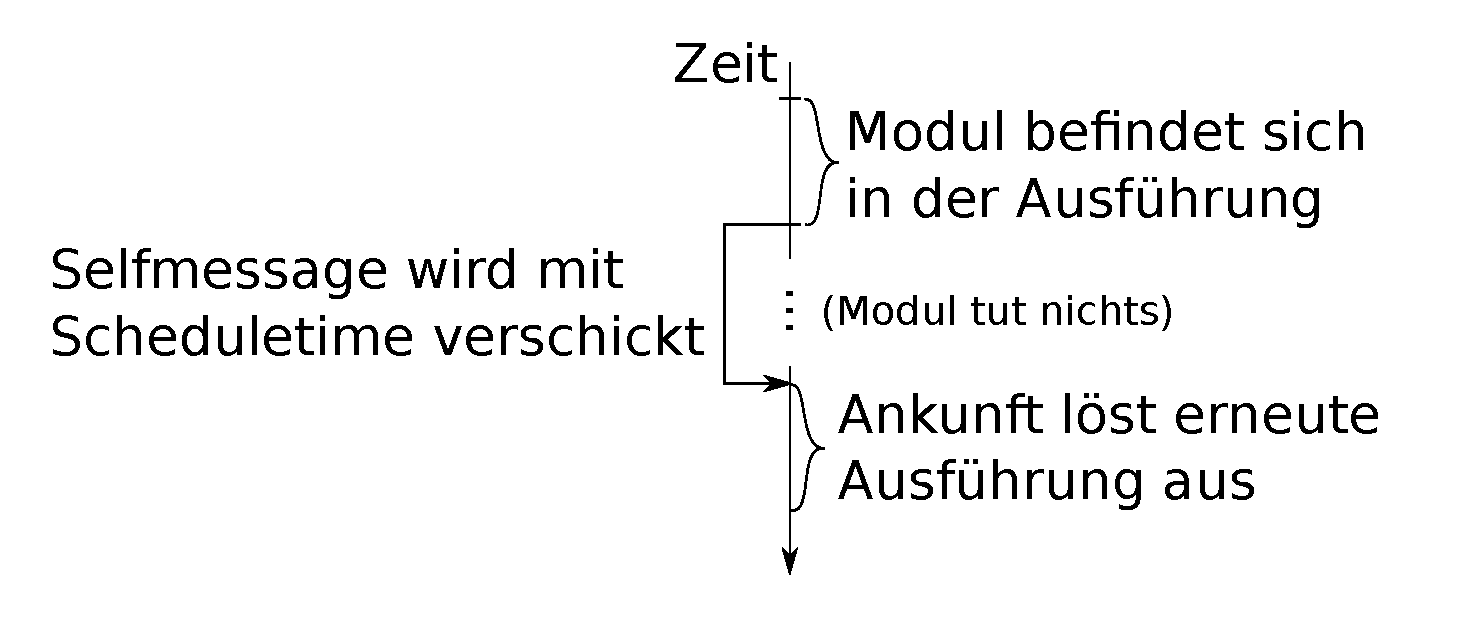
\includegraphics[width=0.8\textwidth]{messageEvent}
\end{figure}

Die Simulationszeit hat den Typ simtime\_t. Im Listing \ref{lst:simtime} sind Beispiele beschrieben, auf welche Weise die aktuelle Zeit abgefragt werden kann und wie ein Event zu einem bestimmten Zeitpunkt ausgelöst werden kann. Dabei kann einfach ein beliebiger Wert als Verzögerung gewählt werden. Dieser wird zur momentanen Zeit addiert und dann wird der Event in Auftrag gegeben.

\begin{minipage}{\textwidth}
\begin{lstlisting}[language=C++,caption={Simulationszeit und Event},label=lst:simtime]
//get the simtime
simtime_t time = simTime();
//define a delay
simtime_t delay = 10.0;
//schedule an event at a given time
scheduleAt(simTime()+delay, event);
\end{lstlisting}
\end{minipage}

\paragraph{cArray} Ist eine Klasse, die als Sammlung für Objekte vom Typ cObject dient. Sie kommt zum Beispiel innerhalb der cMessage zum Einsatz. Die Parameterliste der Nachrichten besteht aus einem solchen cArray. Die wichtigsten Funktionen sind hier add() und remove(), die in Listing \ref{lst:carray} kurz an einem Beispiel gezeigt werden.

\begin{minipage}{\textwidth}
\begin{lstlisting}[language=C++,caption={cArray add und remove},label=lst:carray]
//adding object
cMessage *newmsg = new cMessage("any name");
SimpleCoord *coord = new SimpleCoord("pos", position);
newmsg->getParList().add(coord);
send(newmsg, "toWorld$o");

//getting (and removing) objects
SimpleCoord *array = (SimpleCoord*) msg->getParList().remove(
"pos");
//double x = par->x;
//double y = par->y;
string name = msg->getName();
delete msg;
delete array;

\end{lstlisting}
\end{minipage}

Weiterhin gibt es noch Funktionen wie size(), find() oder clear(), die selbsterklärend sind. Neben remove() gibt es auch noch die Möglichkeit per get() auf Elemente zuzugreifen, ohne sie dabei sofort zu entfernen.

\section{MiXiM-Framework als Omnet++-Erweiterung}

\subsection{Einleitung}

MiXiM\cite{mixim} ist ein Framework welches die Funktionalität von Omnet++ in erster Linie um mobile und kabellose Knoten erweitert. Es implementiert einige Protokolle und stellt verschiedene Knoten bereit.\\
Außerdem fügt es zusätzlich auch nützliche Hilfsfunktionen zu Omnet++ hinzu, wie beispielsweise die FindModule-Klasse.

\subsection{Einige wichtige Module}

\subsubsection{FindModule}

Diese Klasse kann eine Instanz eines Objekts anhand eines Modulnamens finden. Es verhält sich daher wie eine Art Servicemanager. Mann kann mithilfe Dieser Submodule, globale Module, Hostmodule und Netzwerke finden. Dazu übergibt man einfach an ein Template wie in Beispiel \ref{lst:findmodule} den gewünschten Modulnamen und kann dann eine der Methoden, wie zum Beispiel findSubModule() aufrufen.

\begin{lstlisting}[language=C++, caption={Beispiel FindModule}, label=lst:findmodule]
//template der FindModule Klasse
template<typename T = cModule * const >
//Beispielverwendung
FindModule<BasePhyLayer*>::findSubModule(this)
\end{lstlisting}

\subsubsection{Coord}

Coord ist eine einfache Klasse zur Repräsentation von Koordinaten im 3-dimensionalen Raum. Es ist eine elementare Klasse für das MiXiM-Framework, da dieses Mobilität implementiert. Coord beinhaltet zusätzlich zu den 3-D-Koordinaten auch beispielsweise untere und obere Grenzen, Operatoren zum Rechnen und vergleichen und weitere Methoden wie zum Beispiel eine Distanzberechnung zwischen Koordinaten.

\subsubsection{Mobility}

Wie im vorherigen Abschnitt schon erwähnt ist die Mobilität eine der wichtigsten Funktionen, die das MiXiM-Framework bereitstellt. Es werden 4 verschiedene Arten von Bewegungen zur Verfügung gestellt, wobei eine davon, die LineSegmentMobilityBase, selbst wiederum viele verschiedene Varianten zur Verfügung stellt: 
\begin{itemize}
\item CircleMobility
\item LinearMobility
\item RectangleMobility
\item LineSegmentMobilityBase
\end{itemize}
Während die ersten 3 Arten sich von selbst erklären, ist dass bei der LineSegmentMobilityBase nicht der Fall. Es ist eine weitere Basisklasse für Bewegungsarten, welche aus einer Sequenz verschiedener linearer Bewegungen bestehen. Ein Beispiel ist die sogenannte TurtleMobility. Bei dieser kann ein Skript als XML-File hinterlegt werden, welches die Sequenz beschreibt. 

	\chapter{Implementierung}

\section{Einleitung}

Ziel dieser Arbeit war es, eine Simulationsumgebung für Sensorknoten zu schaffen. Es sollte viele verschiedene Arten von Sensorknoten geben, die jeweils einen oder mehrere verschiedene Sensoren besitzen. Mit diesen Knoten sollte ein Netzwerk aufgebaut werden, um die Umgebungsparameter eines Gebietes zu erfassen.
Die Daten der Simulation sollten visualisiert und ausgewertet werden können, besonders was den Energieverbrauch und die dazugehörigen Batteriezustände im Verlauf der Zeit angeht.

\section{Aufbau und Struktur}

\subsection{Klassenübersicht}

Die Klassenübersichten wurden teilweise mit Hilfe von doxygen\cite{doxygen} erstellt. Die Tabelle \ref{Klassenübersicht} zeigt einen Überblick über die definierten Module.

\begin{table}[!ht]
  \centering
  \caption{Klassenübersicht}
  \label{Klassenübersicht}
\begin{tabularx}{\textwidth}{ll}
	\toprule
	Klasse & Beschreibung \\
	\midrule\midrule
	BatteryAccess &	\specialcell{gibt einer Klasse, welche von dieser erbt Zugriff auf \\die Batterie} \\\midrule
Memory & \specialcell{eine einfache Implementierung eines \\key-value-Speichers mit CRUD-Operationen}\\\midrule
Processor	& \specialcell{Repräsentiert ein paar Grundfunktionen eines \\ Prozessor übernimmt die Steuerung der Sensoreinheit, \\ hat Zugriff auf den Speicher und  kann \\außerdem zwischen verschiedenen power-Modi wechseln }\\\midrule
AbstractSensingUnit & \specialcell{einfache Implementierung einer SensingUnit \\ diese kann Werte der Umgebung messen und \\verbraucht dabei Energie}\\\midrule
SensorNode	& \specialcell{ist hauptsächlich für die Initialisierung zuständig}\\\midrule
AbstractSignalConditioner	& modelliert den Energieverbrauch vom SignalConditioner \\\midrule
AbstractSignalConverter	& modelliert den Energieverbrauch vom SignalConverter\\\midrule
AbstractTransducer	& modelliert den Energieverbrauch vom Transducer\\\midrule
CustomWorldUtility	& \specialcell{stellt die Umgebung dar:\\ generiert Umweltparameter und speichert diese\\ liefert auf Anfrage von Sensoren Messwerte}\\\midrule
ExtendedMessage & Nachricht mit einigen Parameters für Statistiken\\\midrule
SimpleSensorData	& \specialcell{eine Klasse die von cNamedObject erbt\\ kann eingesetzt werden um an die Parameterliste \\von Nachrichten angehängt zu werden\\mit dieser können Integerwerte versendet werden}\\\midrule
StatisticsInterface & Interface welches Statistiken zur Verfügung stellt\\
	\bottomrule
\end{tabularx}
\end{table}

\subsubsection{CustomWorldUtility}

Die Klasse CustomWorldUtility ist eine sehr wichtige für die Simulation. Sie repräsentiert die Umgebung, also den Bereich indem sich die Knoten befinden. Sie erbt von der Klasse BaseWorldUtility aus dem MiXiM-Framework. BaseWorldUtility stellt die nötigen Funktionalitäten für den sogenannten Playground bereit. \newline
Zusätzlich dazu stellt die Klasse selbst die notwendigen Parameter für die Umwelt bereit. Nach dem Starten der Simulation steht darin jeweils ein k-dimensionales Array pro Sensortyp bereit: temperatureArray, pressureArray, humidityArray und lightArray. Dabei ist k die definierte Anzahl der Dimensionen, jenachdem ob eine 2-dimensionale Fläche oder ein 3-dimensionaler Raum simuliert werden soll. Die Arrays enthalten die Parameter der Umgebung; temperatureArray beinhaltet zum Beispiel, wie der Name schon sagt, Informationen über die Temperatur. \newline
Es kann zu Beginn der Simulation entschieden werden, ob neue Werte berechnet werden sollen oder die bereits vorhandenen Werte für die Umgebung übernommen werden sollen. Die Arrays besitzen die gleiche Größe wie der Playground. Diese Größe ist auch zusätzlich in den Parametern sizeX, sizeY und sizeZ gespeichert. \newline
Da jedoch im 3-dimensionales Fall die Datenmenge sehr schnell steigt, ist auch möglich über den Paremeter dataGranularity im zugehörigen ned-Modul zu definieren, wie detailliert die Daten erstellt werden sollen. Sollte man zum Beispiel den Wert 10 setzen, so wird nur alle 10 Meter ein Wert generiert.\\
Wenn neue Werte generiert werden sollen, so wird für jeden Messtyp eine xml-Datei in der entsprechenden Größe angelegt und mit Messdaten gefüllt. Diese werden anschließend ausgelesen und in Form der oben genannten Arrays gespeichert. Wenn keine neuen Daten erstellt werden sollen, so wird ein bereits existierendes xml-File genutzt.\\
Zum Erstellen neuer Daten kann die Funktion \textbf{generateEnvironmentData()} genutzt werden. Es ist dadurch auch möglich während der Simulation neue Werte zu generieren, indem man diese Funktion aufruft. Die Funktion legt pro Umweltparameter eine xml-Datei im Ordner \textit{WorldModel/data} an. Jede der xml-Dateien wird beim Start mit Hilfe der Funktion \textbf{readXML(int)} eingelesen, verarbeitet, das heißt in ein Array umgewandelt und anschließend in der Klasse gespeichert. \newline
Sollte nun ein Sensor einen Messwert auslesen wollen, so kann dieser auf die Funktion \textbf{getValueByPosition((std::string type, Coord *position))} zugreifen und anhand seines Sensortyps und seiner Position einen entsprechenden Wert geliefert bekommen.

\paragraph{Einblick in einige Funktionen}

Wie im vorigen Abschnitt beschrieben übernimmt die Funktion generateEnvironmentData() das Erstellen von Umweltparametern. Dafür ruft sie, je nach Sensordatentyp, eine der folgenden Funktionen auf:

\begin{multicols}{2}
\begin{itemize}
\item generateTemperature() - $^\circ $C
\item generatePressure() - hPa
\item generateHumidity()- \%
\item generateLight() - lx
\end{itemize}
\end{multicols}

Diese Funktionen generieren je ein 2- oder 3-dimensionales Array in der Größe des Playgrounds mit Werten, die die jeweils oben angegebenen Einheiten besitzen. In Listing \ref{lst:generateTemp} ist die generateTemperature()-Funktion als ein Beispiel aufgeführt. Im Falle dieser Funktion werden Zufällige integer-Werte generiert, welche sich im Bereich 10 bis 30 bewegen. Dieser erste Entwurf ermöglicht es erst einmal, dass einfach und halbwegs realitätsnahe Werte für den jeweiligen Umweltparameter vorliegen. Später kann an dieser Stelle dann auch ein Zugriff auf eine externe Datenbank erfolgen, in der Messwerte gespeichert sind, die in einem realen Gebiet gemessen wurden.

\begin{lstlisting}[language=C++, label=lst:generateTemp, caption=generateTemperature()]
int* CustomWorldUtility::generateTemperature(int size)
{
    int* data = new int[size];
    for (int i = 0; i < size; i++) {
        //10 - 30
        data[i] = (int)((rand() % 100)/5) + 10;
    }
    return data;
}
\end{lstlisting}

\begin{lstlisting}[language=C++, label=lst:readXML, caption=Kurzbeschreibung readXML()]
cXMLElementList nListRows = rootE->getChildren();
int count = nListRows.size();
for (int i = 0; i < count; i++){
    val[i] = atoi(nListRows[i]->getNodeValue());
}
\end{lstlisting}

Um eben diese Daten wieder lesen zu können dient die Funktion \textbf{readXML()}. Sie verwendet die cXMLElement-Funktionen aus dem Omnet++-Framework. Diese sind sehr hilfreich beim Verarbeiten von XML-Dateien. Ein Bespiel für die Verwendung bei einem XML-File mit einer Verschachtelungstiefe von 1 ist im Listing \ref{lst:readXML} zu sehen. Da in dieser Simulation die Umweltparameter in Form von XML gespeichert sind, ist dies eine sehr nützliche Funktionalität.\\
Die bis jetzt beschriebenen Funktionen dienen alle zur Initialisierung der Simulationsdaten. Es ist natürlich auch möglich diese in einem späteren Verlauf der Simulation erneut aufzurufen und damit neue Werte zu generieren. \\
Für den späteren Verlauf der Simulation ist nun noch die Funktion \textbf{getValueByPosition(std::string, Coord*)} (\ref{lst:getValueByPosition}) von großer Bedeutung. Diese Funktion ermöglich den Sensoreinheiten auf die gespeicherten Daten zuzugreifen.

\begin{lstlisting}[language=C++, label=lst:getValueByPosition, caption=getValueByPosition()]
int CustomWorldUtility::getValueByPosition(std::string type, Coord *position)
{
    int*** data = readXML(getEnumFromType(type));
    int dataAtPosition =
            data
                [(int)(position->x/par("dataGranularity").longValue())]
                 [(int)(position->y/par("dataGranularity").longValue())]
                  [(int)(position->z/par("dataGranularity").longValue())];
    return dataAtPosition;
}
\end{lstlisting}

\subsubsection{SensorNode}

Die Klasse AbstractSensorNode selbst enthält eher weniger Funktionalität. Sie dient hauptsächlich zum initialisieren der gesamten Knotens. Das funktioniert in Omnet++ natürlich zum größten Teil automatisch, allerdings liegt für die Sensoren eine parameterabhängige, generische Initialisierung vor. So können innerhalb den NED-Moduls die folgenden boolschen Parameters gesetzt werden:
\begin{itemize}
\item hasTemperatureSensor
\item hasHumiditySensor
\item hasPressureSensor
\item hasLightSensor
\end{itemize}
Je nachdem ob der jeweilige Parameter gesetzt wird oder nicht wird das entsprechende Sensormodul auf dem Sensorknoten erstellt. Die Gates und Connections eines Moduls lassen sich in der NED-Definition leider nicht so schön generisch erstellen.\\
Daher wird die Initialisierung des Prozessors zusammen mit seinen Gates, Connections und den entsprechenden Channels in der C++-Klasse übernommen. Nach dem Erstellen des Prozessors selbst werden für jeden existierenden Sensor ein eingehendes und ein ausgehendes Gate erstellt. Zusätzlich wird noch ein beidseitiges Gate für die Verbindung zum Memory-Modul angelegt.\\
Die Prozessorgates erhalten dann die Verbindungen zu den jeweils entsprechenden Gates, zum Sensor verläuft ein Gate zur SensingUnit, das vom Sensor eingehende kommt von der Transducer. Beide Verbindungen haben unterschiedliche Funktionen, einmal lediglich zum Senden eines Signals um innerhalb der SensingUnit einen Messvorgang gestartet und ein anderes mal um die gemessenen Werte an den Prozessor zu übermitteln. Es wird daher in 2 verschiedene Channels zum senden unterschieden, welche entsprechend eine höhere oder niedrigere Datenrate aufweisen können, jenachdem wie diese innerhalb des ini-Files definiert sind.\\
Wie genau der Prozessor Schritt für Schritt angelegt wird ist im Listing \ref{lst:initProc} zu sehen. Für das Beispiel wurde jedoch nur ein Paar von Gates verbunden, da das Verbindung für alle anderen Gates analog aussieht.

\begin{lstlisting}[language=C++, label=lst:initProc, caption=teilweise Initialisierung des Prozessors]
//get processor module type
cModuleType *moduleType = cModuleType::get("sensortechnology.src.SensorNode.Processor.Processor");
//create module
cModule *processor = moduleType->create("Processor", this);
processor->finalizeParameters();
//create gate
cGate *fromSensor = processor.addGate(("from" + SensorType + "Sensor").c_str(), cGate::INPUT);
//get sensor
cModule *Sensor = this->getSubmodule((SensorType + "Sensor").c_str());
//get sensor gate
cGate *sensorOut = Sensor->gate("fromTransducerToNodeProcessor");    
//connect the gates
sensorOut->connectTo(fromSensor);    
//finish the process
processor->buildInside();
\end{lstlisting}

\subsubsection{Sensormodule}

Der Sensor in seiner Gesamtheit besitzt keine eigene C++-Klasse. Jedoch besitzt er 4 Module, die gemeinsam die Funktionalität des Sensor ausmachen, welche jeweils eine Klasse haben. Diese werden im folgenden Abschnitt beschrieben.

\paragraph{SensingUnit}

Die SensingUnit ist der wichtigste Teil des Sensors. Innerhalb der Definition von \textbf{handleMessage(cMessage*)} wartet das Modul auf ein Signal vom Prozessor. Sobald dieses kommt wird ein Messvorgang gestartet. Zunächst überprüft das Modul dabei die eigene Position. In Abhängigkeit von dieser wird anschließend ein dem Typ entsprechender Messwert aus dem Modul \textbf{CustomWorldUtility} ausgelesen, welcher hinterher an den SignalConditioner weitergegeben wird. Dazu wird eine Instanz der Klasse SimpleSensorData genutzt, welche an eine cMessage angehängt wird und dann über das entsprechende Gate gesendet wird.

\paragraph{SignalConditioner}

Der SignalConditioner wartet auf eingehende Daten von der SensingUnit. In der Praxis würde das Signal hier aufbereitet werden, jedoch ist die genaue Modellierung an dieser Stelle nicht relevant. Daher kann lediglich ein Energieverbrauch für die durchgeführten Operationen definiert werden, welcher dann bei jedem Aufruf verbraucht wird. Anschließend werden eingegangene Nachrichten weitergeleitet an den SignalConverter.

\paragraph{SignalConverter}

Für den SignalConverter gilt das selbe wie für den SignalConditioner. Die eingegangenen Nachrichten werden lediglich an den Transducer weitergeleitet, ohne das genaue Verhalt zu simulieren und auch dabei steht wieder nur die Modellierung des Energiehaushalts im Vordergrund.

\paragraph{Transducer}

Das letzte Bauteil der Messkette ist der Transducer. Dieser erhält seine Daten vom SignalConverter. Auch hier steht der Energieverbrauch im Vordergrund. Wie in der Realität auch, hat der Transducer am Ende den verwertbaren Messwert in einer festgelegten Einheit vorliegen. Dieser wird anschließend an den Prozessor gesendet, welcher sich dann um die Verwendung dessen kümmert.

\subsubsection{Prozessor}

Eine wichtige Funktion des Prozessors wurde eben schon indirekt beschrieben. Die Klasse \textbf{Processor} kümmert sich um die Steuerung des Sensors. Aber er erfüllt auch andere Funktionen, wie die Energieverwaltung des Sensorknotens und die Verwertung von statistischen Daten.

\paragraph{Sensorsteuerung}

Der jeweilige Prozessor kann über das entsprechende, ausgehende Gate zu seinen Sensoren einen Messvorgang auslösen, indem die Funktion startSensingUnit() (Listing \ref{lst:startSensingUnit}) aufgerufen wird. Anschließend bekommt er die Daten vom Transducer übermittelt. Diese Information kann nun unterschiedlich behandelt werden. Typischer Weise kann dieser Wert nun zunächst im Speicher hinterlegt werden. Dafür wird die eingegangene Message direkt an den Memory weitergeleitet. Wie das genau aussieht ist im folgenden Abschnitt des Memories beschrieben.\\
Es ist auch möglich periodisch Messungen durchzuführen. Dazu muss lediglich im NED-Modul ein Wert für sensingIntervall gesetzt werden. Dieser legt fest, welche zeitlichen Abstände zwischen 2 Messungen vorliegen sollen. Es wird dann bei der Initialisierung ein Event gestartet welcher jeweils nach dem festgelegten Zeitintervall ausgelöst wird. In diesem Fall wird dann ein Messvorgang gestartet. Danach wird der nächste folgende Event initialisiert und zum gegebenen Zeitpunkt beginnt der Vorgang von neuem.

\begin{lstlisting}[language=C++, label=lst:startSensingUnit, caption=startSensingUnit()]
void Processor::startSensingUnit()
{
    cModule* SensorNode = getParentModule();
    if (SensorNode->par("hasTemperatureSensor")) {
        cMessage* msg = new cMessage("startMeasuring");
        send(msg, "toTemperatureSensor");
    }
    if (SensorNode->par("hasHumiditySensor")) {
        cMessage* msg = new cMessage("startMeasuring");
        send(msg, "toHumiditySensor");
    }
    if (SensorNode->par("hasPressureSensor")) {
        cMessage* msg = new cMessage("startMeasuring");
        send(msg, "toPressureSensor");
    }
    if (SensorNode->par("hasLightSensor")) {
        cMessage* msg = new cMessage("startMeasuring");
        send(msg, "toLightSensor");
    }
}
\end{lstlisting}

\paragraph{ProcessorMode}

Weiterhin hat der Prozessor die Möglichkeit zwischen verschiedenen Powermodi zu wechseln. Die existierenden Modi sind in einem enum (Listing \ref{lst:ModeEnum}) definiert und können per Funktion switchProcessorMode gewechselt werden (Listing \ref{lst:switchProcessorMode}).

\begin{lstlisting}[language=C++, label=lst:ModeEnum, caption=enum MODES]
enum MODES { 
	NORMAL = 0, 
	POWER_SAVING = 1, 
	HIGH_PERFORMANCE = 2, 
	OFF 
}
\end{lstlisting}

\begin{lstlisting}[language=C++, label=lst:switchProcessorMode, caption=switchProcessorMode()]
void Processor::switchProcessorMode(MODES mode)
{
    //switch batteries power accounts
    if (mode == POWER_SAVING) {
        drawCurrent(currentOverTimePowerSaving, 1);
    } else if (mode == NORMAL) {
        drawCurrent(currentOverTimeNormal, 0);
    } else if (mode == HIGH_PERFORMANCE) {
        drawCurrent(currentOverTimeHighPerformance, 2);
    }
}
\end{lstlisting}

So können beispielsweise Tagesabläufe der Sensorknoten gesteuert werden. Da die Energiequelle von Sensorknoten oft sehr klein ist, ist es sinnvoll die Knoten in Zeiten, in denen keine Messwerte aufgenommen werden sollen in einen Stand-By Zustand zu versetzen. Dadurch kann viel Energie gespart werden.\\
Diese Funktion wird durch die verschiedenen Powermodi bereitgestellt. Es ist möglich einen Zeitintervall zu definieren, in dem die verschiedenen Knoten gemeinsam zwischen den verschiedenen Modi wechseln. Da ein Knoten in Zeiten des Stand-By keine Kommunikation durchführen kann, ist am sinnvollsten alle Knoten im Netzwerk synchron schlafen zu lassen. Der entsprechende Zeitintervall kann durch die Variable shiftProcessorModeIntervall definiert werden.\\
Dadurch werden nun wieder zeitlich periodische Wechsel zwischen den Modi durchgeführt, welche durch Events gesteuert werden, indem die Funktion switchProcessorMode() (\ref{lst:switchProcessorMode}) aufgerufen wird. Diese Funktion ist überladen und kann auf 3 verschiedene Arten aufgerufen werden: mit dem Modus in die gewechselt werden soll, mit dem int-Wert der diesen Modus repräsentiert oder ohne Parameter, in dem Fall wird der nächste Modus anhand der Integerwerte bestimmt, wie bei einem Modulozähler.\\
Für jeden einzelnen Zustand kann dann wiederum im ini-File definiert werden, wie der Energieverbrauch pro Zeiteinheit während welches Modus genau aussehen muss.

\paragraph{Statistiken}

Die dritte Funktion des Prozessors, welche ebenfalls über Events gesteuert wird, ist das Erfassen statistischer Daten. Auch hierfür kann, in Form von der Variable collectStatisticsIntervall, ein zeitlicher Intervall definiert werden, nach diesem jeweils ein Event eine Erhebung von statistischen Messwerten des Batteriezustands durchführt. Die dazu gehörige Funktion ist in Listing \ref{lst:doCollectStatistics} zu sehen.

\begin{lstlisting}[language=C++, label=lst:doCollectStatistics, caption=doCollectStatistics()]
void Processor::doCollectStatistics()
{
    voltage = battery->getVoltage();
    voltageStats.collect(voltage);
    voltageVector.record(voltage);

    residualRelative = battery->estimateResidualRelative();
    residualRelativeStats.collect(residualRelative);
    residualRelativeVector.record(residualRelative);

    residualAbs = battery->estimateResidualAbs();
    residualAbsStats.collect(residualAbs);
    residualAbsVector.record(residualAbs);
}
\end{lstlisting}
\subsubsection{Memory}

Der Speicher besitzt arrays für einen key-value-Speicher und implementiert zur Benutzung dieses Speichers die CRUD-Operationen, wie in Listing \ref{lst:CRUD} zu sehen ist.

\begin{lstlisting}[language=C++, label=lst:CRUD]
#define error -9999
const static int storageSize = 4;

void Memory::createEntry(std::string type, int value)
{
    int emptyId = -1;
    for (int i = 0; i < storageSize; i++) {
        if (storageType[i] == "") {
            emptyId = i;
            break;
        }
    }
    if (emptyId == -1) {
        return;
    }
    storageType[emptyId] = type;
    storageValue[emptyId] = value;
}

int Memory::readEntry(std::string type)
{
    int id = getIdByType(type);
    if (id == -1) {
        return error;
    }
    return storageValue[id];
}

void Memory::updateEntry(std::string type, int value)
{
    int id = getIdByType(type);
    if (id == -1) {
        return createEntry(type, value);
    }
    storageValue[id] = value;
}

void Memory::deleteEntry(std::string type)
{
    int id = getIdByType(type);
    if (id == -1) {
        return;
    }
    storageValue[id] = error;
    storageType[id] = "";
}
\end{lstlisting}

Wenn nun von außen eine Message mit einem Datensatz an den Speicher geschickt wird, so kann dieser je nach Bedarf Datensätze neu anlegen, löschen oder updaten, damit diese später, wenn die Daten benötigt werden, wieder abgerufen werden können.

\subsubsection{BatteryAccess}

Die Klasse BatteryAccess ermöglicht den Modules des Sensors auf die Batterie zugreifen zu können. Dafür ist zunächst eigentlich die Klasse MiximBatteryAccess zuständig. BatteryAccess erbt von dieser und erweitert sie um einige wichtige Funktionen.\\
So können zum Beispiel direkt Werte für den Energieverbrauch des entsprechenden Moduls hinterlegt werden. Immer wenn nun eine Energieintensive Operation durchgeführt wird, verbraucht die Batterie Energie in Höhe dieses definierten Wertes, indem die Funktion draw() aufgerufen wird. Diese ruft anschließend die Funktion drawEnergie(float) mit dem gespeicherten Wert \textbf{float energiePerOperation} auf.\\
Die Klasse kümmert sich weiterhin um die Initialisierung und um den Fall, dass die Batterie den leeren Zustand erreicht (handleHostState()).

\begin{lstlisting}[language=C++, label=lst:BatteryAccess]
class BatteryAccess : public MiximBatteryAccess {
protected:
    float currentOverTime;
    float energiePerOperation;
    //int deviceID; - defined inside MiximBatteryAccess
public:
    BatteryAccess();
    virtual ~BatteryAccess();
    void initialize(int stage);
    void draw();
    void finish();
    virtual void handleHostState(const HostState &state);
};
\end{lstlisting}

\subsubsection{SimpleSensorData}

\begin{figure}[htbp]
\centering
\caption{SimpleClasses: Member}
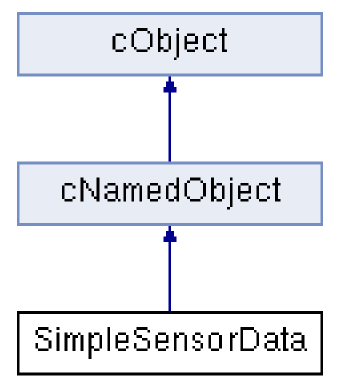
\includegraphics{SimpleClasses}
\end{figure}

\begin{lstlisting}[language=C++, label=lst:SimpleExample]
//im Sender:
cMessage *msg = new cMessage(msgname);
SimpleSensorData *data = new SimpleSensorData("Temperature", temp);
msg->getParList().add(coord);

//
// Nachricht uebertragen    
//  
  
//im Empfaenger:  
SimpleSensorData *data = (SimpleSensorData*) msg->getParList().remove("Temperature");
\end{lstlisting}

\subsubsection{ExtendedMessage}

ExtendedMessage erbt direkt von der Klasse cMessage, der Standard-Nachrichtenklasse in Omnet++. Im Grunde stellt cMessage alle benötigten Funktionen bereit. ExtendedMessage ist nur aus dem Grund vorhanden, um zusätzliche Statistiken über Nachrichten erstellen zu können, zum Beispiel wie oft eine einzelne Nachricht weitergesendet wurde.

\begin{figure}[htbp]
\centering
\caption{ExtendedMessage: Vererbung}
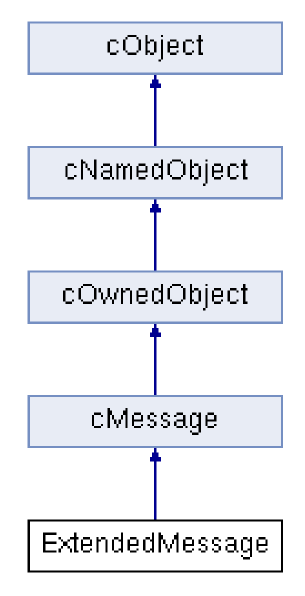
\includegraphics{ExtendedMessage}
\end{figure}

Im Listing \ref{lst:ExtendedMessage} ist zu sehen welche Statistikparameter erhoben werden.

\begin{minipage}{\textwidth}
\begin{lstlisting}[language=NED, label=lst:ExtendedMessage]
message ExtendedMessage extends cMessage
{
    int source;
    int destination;
    int hopCount = 0;    
}
\end{lstlisting}
\end{minipage}

\subsubsection{StatisticsInterface}

Dieses Interface enthält grundlegende Attribute für Statistiken. Klassen die dieses implementieren speichern somit zum Beispiel wie viele Nachrichten sie empfangen oder gesendet haben.

\subsection{Übersicht NED-Module}

Im folgenden Abschnitt werden alle Simulationsobjekte erläutert, also all jene, die durch die Sprache NED beschrieben wurden:

\begin{minipage}{\textwidth}
\begin{itemize}{\label{enum:NedModules}}
\item Simple Module
\begin{multicols}{2}
\begin{itemize}
\item AbstractSensingUnit
\item AbstractSignalConditioner
\item AbstractSignalConverter
\item AbstractTransducer
\item CustomWorldUtility
\item ExampleProcessor
\item Memory
\item Processor
\item SensingUnitHumidity
\item SensingUnitLight
\item SensingUnitPressure
\item SensingUnitTemperature
\item SignalConditionerHumidity
\item SignalConditionerLight
\item SignalConditionerPressure
\item SignalConditionerTemperature
\item SignalConverterHumidity
\item SignalConverterLight
\item SignalConverterPressure
\item SignalConverterTemperature
\item TransducerHumidity
\item TransducerLight
\item TransducerPressure
\item TransducerTemperature 
\end{itemize}
\end{multicols}
\item Compound Module
\begin{multicols}{2}
\begin{itemize}
\item AbstractSensor
\item SensorNode
\item HumiditySensor
\item LightSensor
\item PressureSensor
\item TemperatureSensor 
\end{itemize}
\end{multicols}
\item Messages und Channel
\begin{multicols}{2}
\begin{itemize}
\item ExtendedMessage
\item DatarateChannel
\end{itemize}
\end{multicols}
\end{itemize}
\end{minipage}

\subsubsection{Simple Module}

Simple Module sind Komponenten in einer Omnet++ Simulation, die die größte Auswirkung auf die Wirkungsweise des Netzwerkes haben. Das liegt daran, dass bei ihnen neben einer Beschreibung in NED auch eine Beschreibung in C++ vorliegt. Daher kann das Verhalten jener Module während der Simulation ausführlich definiert werden. Simple Module werden oft in Gruppen zusammengefasst, also in Compound Modulen. Dadurch kann man komplexe Modellbeschreibungen erzeugen.\\
Im folgenden Teil werden einige dieser Simple Module beschrieben.

\subsubsection{CustomWorldUtility}

Wie im Codebeispiel (\ref{lst:CustomWorldUtility}) zu sehen ist, ist das Modul CustomWorldUtility eine Erweiterung des Moduls BaseWorldUtility. Zusätzlich zu den darin definierten Eigenschaften hat es einige weitere Parameter. Zum einen den integer-Wert dataGranularity, welcher festlegt, wie genau die Messwerte generiert werden sollen. Er legt fest, wie groß die Fläche, beziehungsweise  der Würfel sein soll, für die jeweils ein Messwert angelegt wird. Dabei definiert dataGranularity die Kantenlänge. Die restlichen Variablen speichern die Speicherorte für die Messwerte, welche als xml-Datei erstellt werden.

\begin{minipage}{\textwidth}
\begin{lstlisting}[language=ned,caption={CustomWorldUtility},label=lst:CustomWorldUtility]
package mynetwork.WorldModel;
import org.mixim.base.modules.BaseWorldUtility;

simple CustomWorldUtility extends BaseWorldUtility
{
    bool createData;
        int dataGranularity;
        string basePath = "src/WorldModel/data/";
        xml xmlTemperature = xmldoc("src/WorldModel/data/temperature.xml");
        xml xmlPressure = xmldoc("src/WorldModel/data/pressure.xml");
        xml xmlHumidity = xmldoc("src/WorldModel/data/humidity.xml");
        xml xmlLight = xmldoc("src/WorldModel/data/light.xml");
        @class("CustomWorldUtility");
}
\end{lstlisting}
\end{minipage}

\subsubsection{Sensormodule}

Es gibt 4 verschiedene Module aus denen sich ein Sensor, unabhängig von seinem Typ, zusammen setzt:

\begin{itemize}
\item SensingUnit
\item SignalConditioner
\item SignalConverter
\item Transducer
\end{itemize}

Für jeden dieser Typen gibt es ein abstraktes Modell, von welchem alle Sensortypen mit einer eigenen Implementierung erben. Weiterhin steht ein Interface zur Verfügung, welche diese implementieren müssen. Unterschiedliche Parameter besitzen die einzelnen Implementierungen nicht, jedoch bieten die verschiedenen Benennungen die Möglichkeit, den Energieverbrauch für jeden unterschiedlichen Sensortyp genau steuern zu können.\\
Alle dieser Module haben jeweils Parameter für den Energieverbrauch, welcher in der dahinter liegenden Klasse ausgewertet wird und ein input und ein output Gate. Die Verbindungen zu denen die Gates führen unterscheiden sich jedoch.\\
Während für die in der Messkette mittleren Module jeweils ein Gate zum vorherigen und eines zum nachfolgenden Modul führt, gilt das nicht für die SensingUnit und den Transducer. Die SensingUnit hat ein eingehendes Gate vom Prozessor, welcher ein Signal senden kann, um eine Messung in Gang zu setzen und der Transducer besitzt ein ausgehendes Gate zum Prozessor, um die fertig eingelesenen Daten an diesen zu übermitteln.

\subsubsection{Prozessor}

Das NED-Modul des Prozessors bietet nicht besonders viele Einstellungsmöglichkeiten. Es existiert ein Parameter numGates, welcher definiert, wie viele Gates der Prozessor besitzt, wobei der Wert dafür innerhalb der Initialisierung der C++-Klasse gesetzt wird. Zusätzlich kann die Anzahl der Prozessor Modi geändert werden, wobei dann wiederum zusätzliche Anpassungen innerhalb der C++-Klasse notwendig sind, damit diese auch genutzt werden können. Weiterhin können für die bestehenden 3 Modi die Parameter für den Energieverbrauch jeweils definiert werden.

\subsubsection{Memory}

Das NED-Modul des Speichers bietet nicht viele Parameter. Lediglich der Energieverbrauch des Bauteils kann an dieser Stelle definiert werden.

\subsubsection{Compound Module}

Compound Module dienen dazu, andere Module zusammenzufassen, sollen jedoch keine eigene aktive Funktionalität definieren. Ihr Verhalten soll sich allein durch die Submodule ergeben. Es ist daher nicht sinnvoll eine C++-Klasse für diese Module zu definieren.\newline
Für den Sensorknoten wurde dennoch eine eigene Klasse definiert, welche allerdings keine Funktion während der Simulation übernimmt, sondern allein für die generische Initialisierung zuständig ist.

\subsubsection{Sensoren}

\begin{figure}[htbp]
\centering
\caption{allgemeines Modell eines Sensors}
\label{fig:SensorModel}
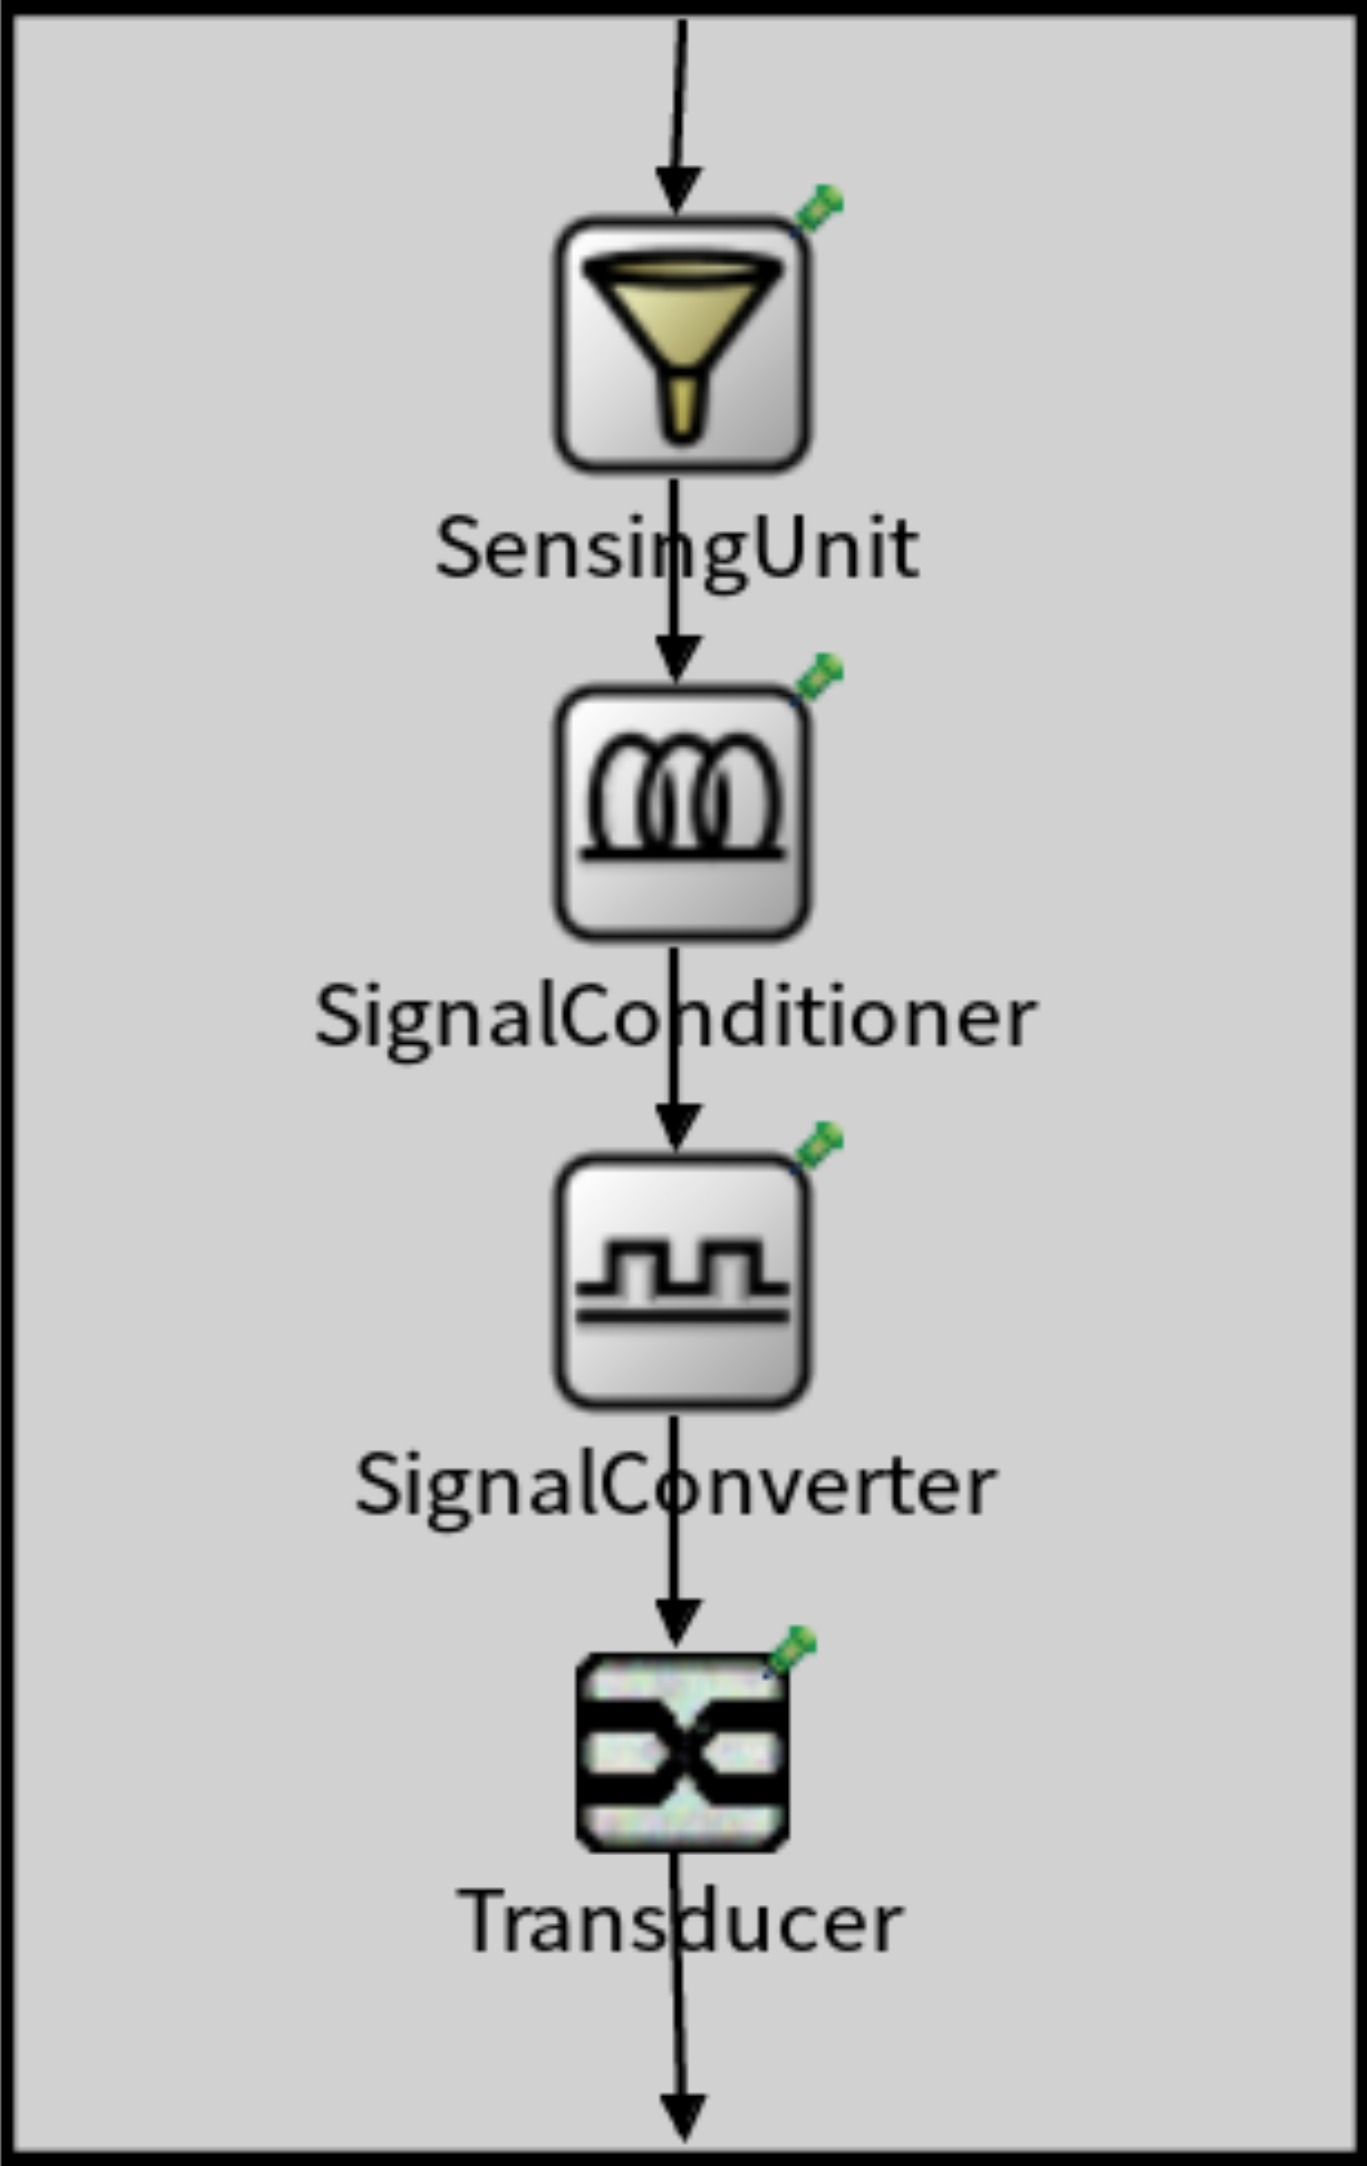
\includegraphics[]{SensorModel}
\end{figure}

Es liegt ein abstraktes Modul und ein Modulinterface für die verschiedenen Sensoren vor und für jeden Sensortyp existiert ein Sensormodul, welches vom abstrakten Modul erbt und das Sensorinterface implementiert.\\
Die Abstrakte Klasse besitzt wenige Parameter; zum einen type, in dem in der jeweiligen Sensorimplementierung der Typ des Sensors definiert werden muss und die beiden Parameter dataBandwidth und controlBandwidth, welche die Bandbreite für die 2 verschiedenen Arten von Channels definieren.\\
Das wichtigste ist natürlich die Definition der Submodule (\ref{lst:AbstractSensor}), denn diese machen die Funktionalität eines Compound Moduls aus. Die Abbildung \ref{fig:SensorModel} zeigt diesen Aufbau in bildlicher Form.

\begin{lstlisting}[language=ned,caption={AbstractSensor},label=lst:AbstractSensor]
submodules:
        SensingUnit: <"SensingUnit"+type> like SensingUnitInterface {
            @display("p=100,50");
        }
        SignalConditioner: <"SignalConditioner"+type> like SignalConditionerInterface {
            @display("p=100,120");
        }
        SignalConverter: <"SignalConverter"+type> like SignalConverterInterface {
            @display("p=100,190");
        }
        Transducer: <"Transducer"+type> like TransducerInterface {
            @display("p=100,260");
        }
\end{lstlisting}

Anhand der Submoduldefinition ist auch ersichtlich, weshalb jedes Modul des Sensor jeweils ein Interface implementieren muss. Für das parametrische Anlegen von Submodulen, muss wenigstens ein Interface definiert werden, dem das Modul angehören muss, damit nicht jedes beliebige Modul an dieser Stelle eingesetzt werden kann.

\subsubsection{SensorNode}

\begin{figure}[htbp]
\centering
\caption{Aufbau des Compoundmoduls SensorNode}
\label{fig:Sensornode}
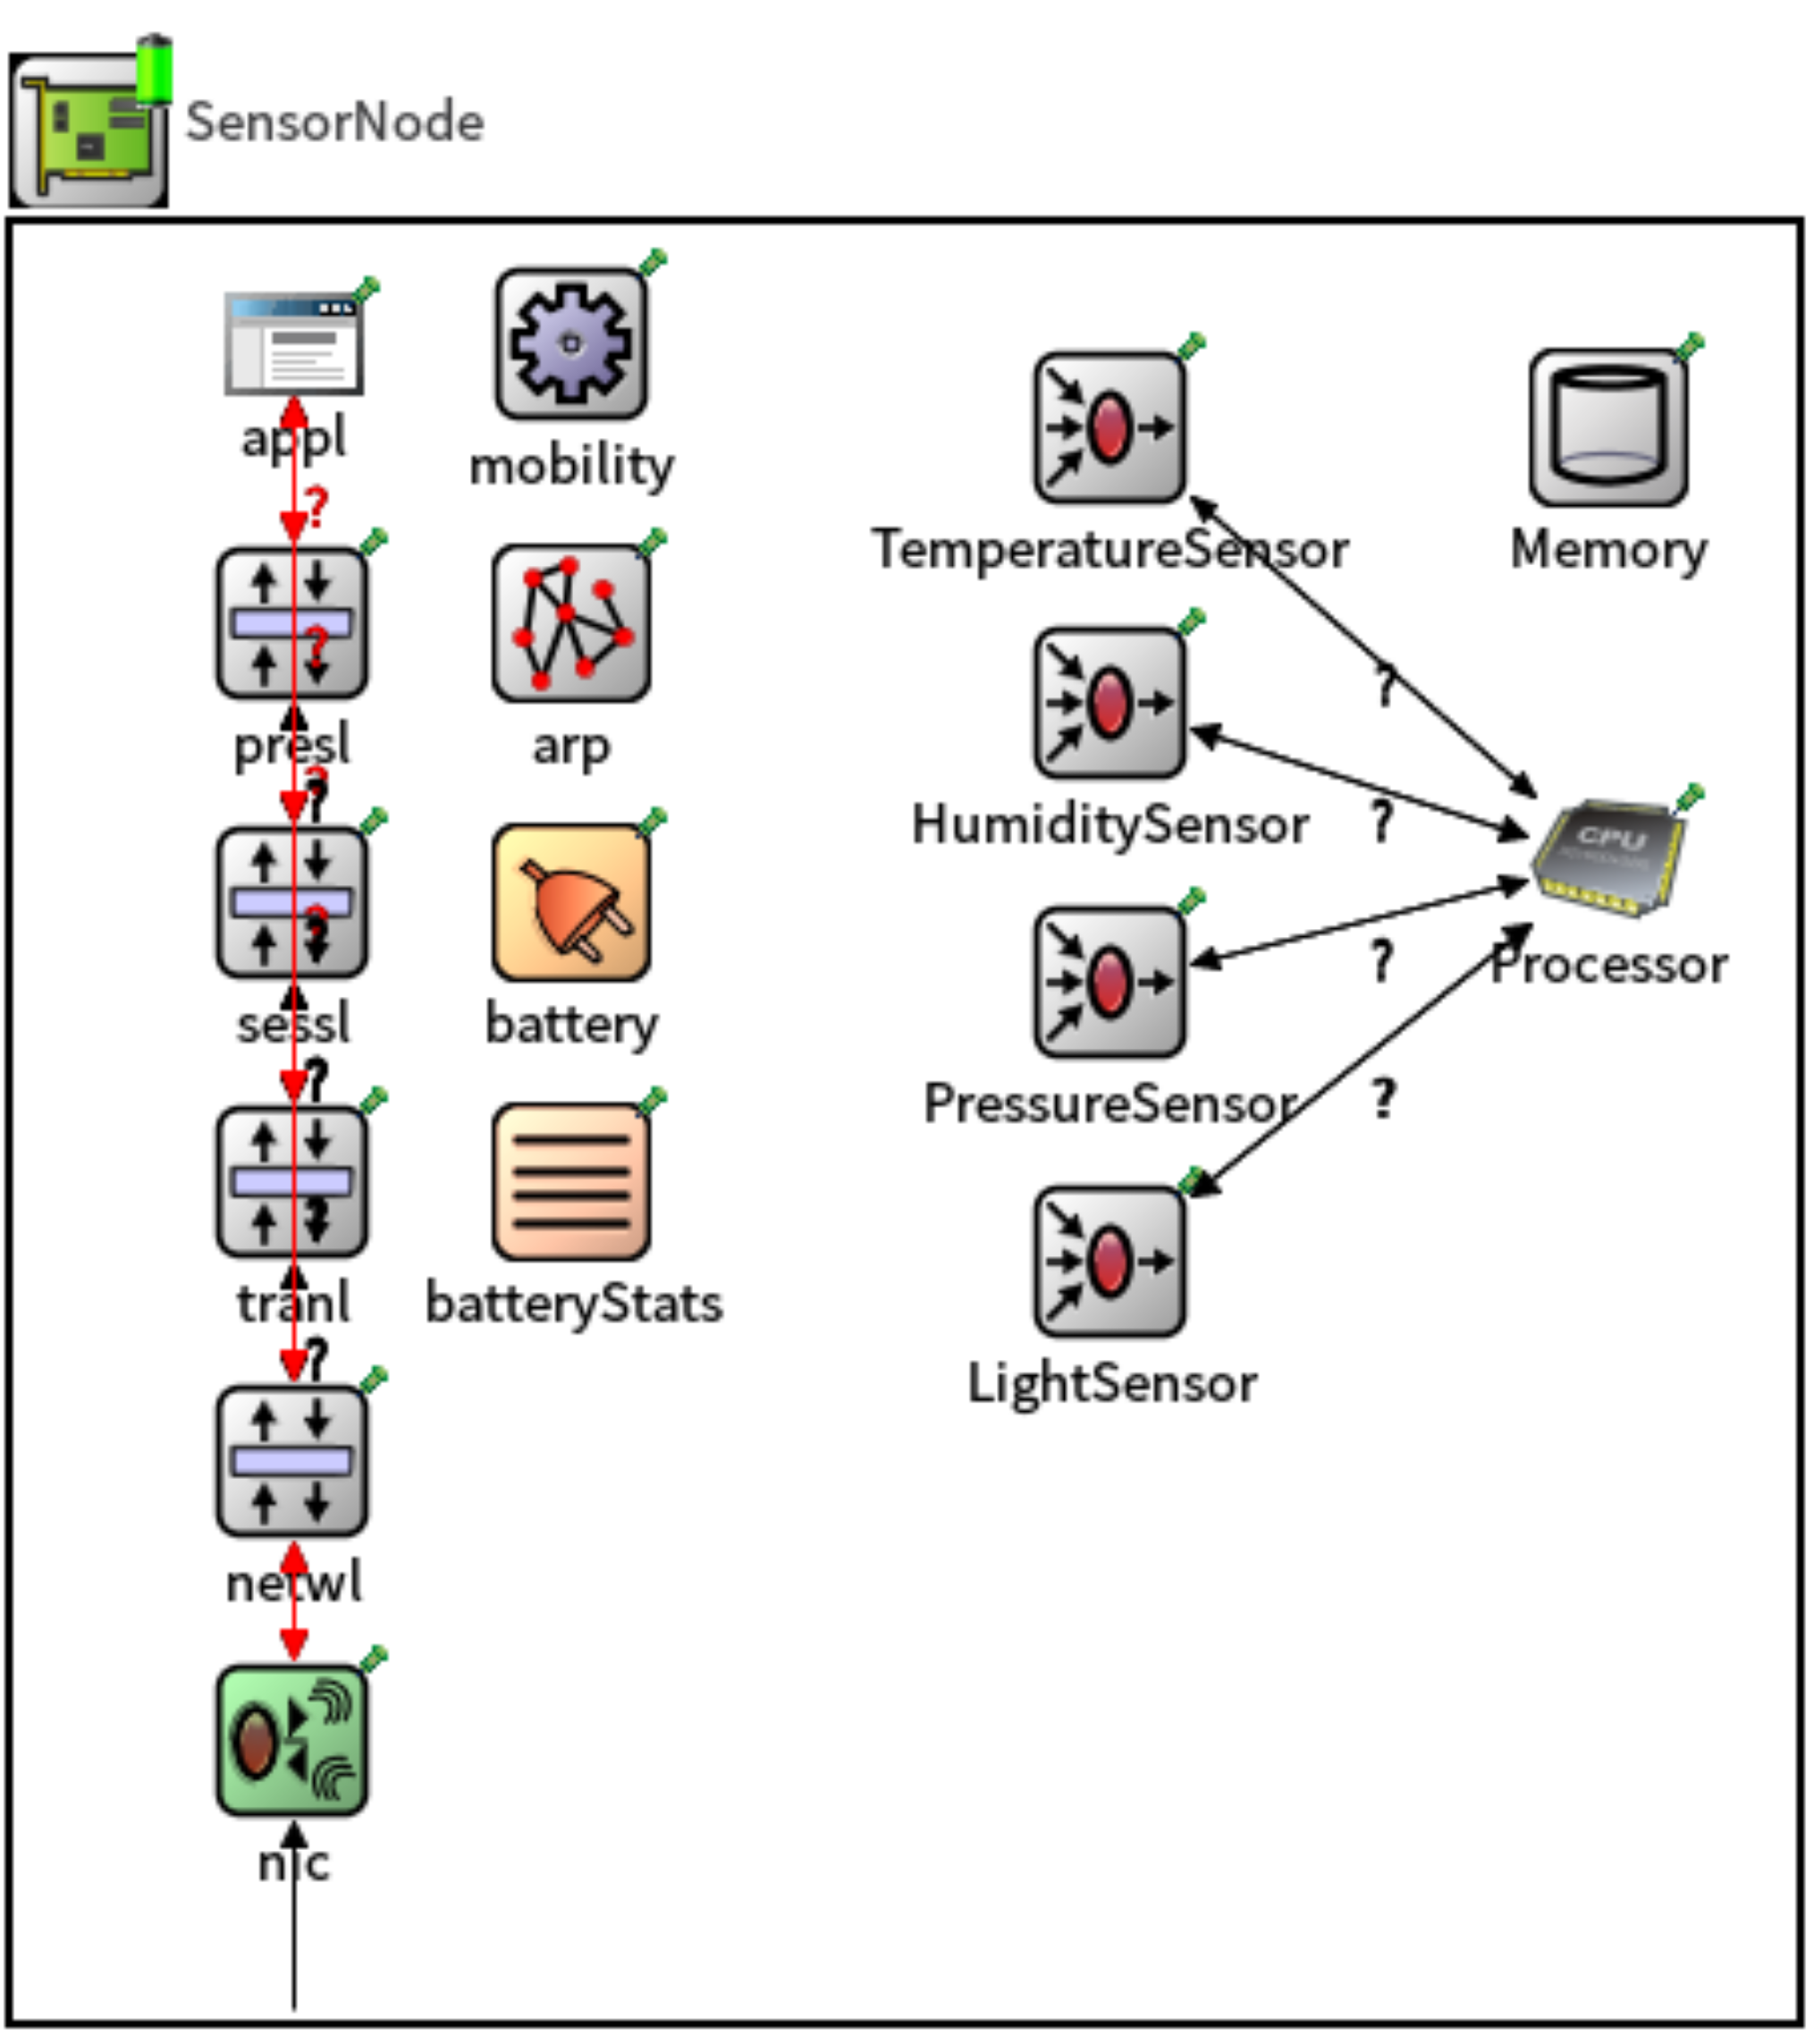
\includegraphics[width=\textwidth]{Sensornode}
\end{figure}

Der SensorNode ist das komplexeste Compound Modul in der Simulation, denn es beinhaltet die bisher beschriebenen Module Sensor, Prozessor, Memory und die in MiXiM enthaltenen Module für die Funkkommunikation und eine Batterie.\\
Die MiXiM-Module werden dem Sensorknoten durch das erben von dem Modul \textbf{WirelessNodeBatteryPlusTran} aus dem MiXiM-Framework zugewiesen, da dieses die benötigte Batterie und die Funkkommunikation bereitstellt. Alle anderen Module werden wie im Beispiel \ref{lst:SensorNode} definiert. Dieses ist dabei auf die Definition der Submodule reduziert.

\begin{lstlisting}[language=ned,caption={SensorNode mit den neu definierten Modulen},label=lst:SensorNode]
module SensorNode extends WirelessNodeBatteryPlusTran like SensorNodeInterface
{
    parameters:
    
        //[...]

    submodules:
        TemperatureSensor: TemperatureSensor if hasTemperatureSensor {
            @display("p=275,51");
            dataBandwidth = dataBandwidth;
            controlBandwidth = controlBandwidth;
        }
        HumiditySensor: HumiditySensor if hasHumiditySensor {
            @display("p=275,120");
            dataBandwidth = dataBandwidth;
            controlBandwidth = controlBandwidth;
        }
        PressureSensor: PressureSensor if hasPressureSensor {
            @display("p=275,190");
            dataBandwidth = dataBandwidth;
            controlBandwidth = controlBandwidth;
        }
        LightSensor: LightSensor if hasLightSensor {
            @display("p=275,260");
            dataBandwidth = dataBandwidth;
            controlBandwidth = controlBandwidth;
        }
        Memory: Memory {
            @display("p=400,51");
        }
        Processor: Processor {
            @display("p=400,159");
        }
        
    connections:
    
        //[...]
        
}        
\end{lstlisting}

Durch das Setzen von hasTemperatureSensor und den analogen boolschen Variablen für die anderen Sensortypen kann für jeden Sensorknoten festgelegt werden, über welche Sensoren er verfügt. Das kann beispielsweise innerhalb der Definition des Netzwerkes geschehen.

\begin{itemize}
\item TemperatureSensor
\item HumiditySensor
\item LightSensor
\item PressureSensor
\end{itemize}

\subsubsection{Messages und Channels}

Nachrichten sind das essentielle Werkzeug, um in einem Netzwerk Kommunikation zu ermöglichen. Es gibt ein vordefiniertes Modul cMessage, welches dafür genutzt werden kann. Dieses beinhaltet notwendige Informationen wie zum Beispiel Sendermodul und -gate, Empängermodul und -gate, Sende-, Empfangs- und Erstellzeit und mehr.

\subsubsection{ExtendedMessage}

Die ExtendedMessage erweitert diese Funktionalität um einige Informationen für die Statistik.

\begin{lstlisting}[language=ned,caption={ExtendedMessage},label=lst:ExtendedMessage]
message ExtendedMessage extends cMessage
{
    int source;
    int destination;
    int hopCount = 0;    
}
\end{lstlisting}

\subsubsection{DatarateChannel}

DatarateChannel ist ein von Omnet++ definiertes Modul. Es kann mit verschiedenen Parametern versehen werden, um dem jeweiligen Umständen angepasst zu werden. Der wichtigste ist dabei der double datarate, welcher in bps angegeben wird und festlegt, mit welcher Rate Daten durch den Channel gesendet werden können. Weiterhin kann auch ein delay und eine bit- beziehungsweise packet-error-rate festgelegt werden.\\
In der Simulation wurde dieses Modul genutzt, um die verschiedenen Kanäle für den Datenverkehr und die Steuerungskanäle zu trennen.

\subsubsection{omnetpp.ini}

Die omnetpp.ini ist eine Datei, in der Eigenschaften der Simulation geändert werden können, ohne das man den Sourcecode bearbeiten und danach neu kompilieren muss. Es bietet sich daher an, alle Variablen und Konstanten, welche sich öfters ändern hier zu definieren. Die wichtigsten Parameter sind im Beispiel \ref{lst:omnetini} aufgeführt.

\begin{lstlisting}[language=ned,caption={wichtige Parameter für das ini-File},label=lst:omnetini]
#Energieverbrauch
**.Memory.currentConsumption = 3
**.Memory.energyConsumption = 100

**.currentConsumption = 5
**.energyConsumption = 150

#capacity = nominal
**.battery.nominal = 1000mAh

#Playground
**.playgroundSizeX = 400m
**.playgroundSizeY = 550m
**.playgroundSizeZ = 100m

#defines how big the edge size of the cube is, a single value will represent
**.dataGranularity = 10

#zero is treated specially: no periodic behavior
#defines the time between two measurings of a sensor
**.sensingIntervall = 10000s
#time between mode shifts
**.shiftProcessorModeIntervall = 5000s
#time between information collections
**.collectStatisticsIntervall = 1000s
\end{lstlisting}

\section{Funktionsweise mit Beispielanwendungen}

All die in diesem Kapitel beschriebenen Module wirken für die Simulation zusammen, um ein Netzwerk aus Sensorknoten zu schaffen, in dem die Knoten miteinander und mit ihrer Umgebung gemeinsam agieren können. Dazu werden nach dem Start der Simulation Umweltparameter bereitgestellt und eine festgelegte Anzahl von verschiedenen Sensorknoten erzeugt. Diese können sich anschließend bewegen oder ihr Position beibehalten. Sie können mit ihren Sensoren Werte der Umgebung erfassen und diese über Funk an andere Sensorknoten übertragen, sollte diese in der näheren Umgebung zur Verfügung stehen.

    %\chapter{Evaluation}

    \chapter{Zusammenfassung}

In der Arbeit wurden verschiedene Module implementiert oder integriert. Dadurch kann ermittelt werden, wie sich verschiedene Eigenschaften des Netzwerks auf die Lebenszeit der Sensorknoten auswirkt. Dazu wurden Modul des Wakeupreceivers, der Sensorik und das ApplicationClustering in ein neues Modul integriert. Zusätzlich wurde das Verhalten der entstandenen Sensorknoten mit Wakeupreceiver in 3 verschiedenen Szenarien implementiert. Dazu wurden zum einen Applicationlayer und zum anderen Networklayer implementiert.\\
In den 3 Szenarien kommen die verschiedenen Layer mit unterschiedlichen Konfigurationen der Knoten und des Netzwerks zum Einsatz. 
	
	%%========================================================================================	
	%% formaler Aufbau - Ende 
	%%========================================================================================
    %\input{formalLayout/arbeitsaufteilung}
	%\manualmark
%\addcontentsline{toc}{chapter}{Glossar}
%\markboth{Glossar}{Glossar}
%\def\glossaryname{Glossar}
%\printglosstex(glo)
%\cleardoublepage
	%\manualmark
\markboth{Literaturverzeichnis}{Literaturverzeichnis}
\def\bibname{Literatur- und Webverzeichnis}
\bibliographystyle{gerplain}
\bibliography{bib/literatur}
\cleardoublepage
	\chapter*{Selbstständigkeitserklärung}
\thispagestyle{empty}	%keine Seitenzahl!
\pdfbookmark{Selbstständigkeitserklärung}{Selbstständigkeitserklärung}

Hiermit erkläre ich, dass ich die vorliegende Arbeit
selbstständig angefertigt, nicht anderweitig zu Prüfungszwecken vorgelegt und
keine anderen als die angegebenen Hilfsmittel verwendet habe. Sämtliche 
wissentlich verwendete Textausschnitte, Zitate oder Inhalte anderer Verfasser 
wurden ausdrücklich als solche gekennzeichnet.\\[2ex]
\dcplace, den \dcdate\\[6ex]
\flushleft
\newlength\us
\settowidth{\us}{-\dcauthorfirstname~\dcauthorlastname-}
\begin{tabular}{p{\us}}\hline
\centering\footnotesize \dcauthorfirstname~\dcauthorlastname
\end{tabular}
	%\part*{Anhang}
\cleardoublepage
\appendix
%\include{anhanga}
	
\nocite{sensornetzwiki}
\nocite{miximapiref}
\nocite{omnetman}	
\nocite{hsc}
\nocite{ns3-wiki}
\nocite{softwarearch}
\nocite{tempsensor}
\nocite{sensor}
\end{document}
